%% uctest.tex 11/3/94
%% Copyright (C) 1988-2004 Daniel Gildea, BBF, Ethan Munson.
%
% This work may be distributed and/or modified under the
% conditions of the LaTeX Project Public License, either version 1.3
% of this license or (at your option) any later version.
% The latest version of this license is in
%   http://www.latex-project.org/lppl.txt
% and version 1.3 or later is part of all distributions of LaTeX
% version 2003/12/01 or later.
%
% This work has the LPPL maintenance status "maintained".
% 
% The Current Maintainer of this work is Daniel Gildea.

\documentclass[11pt]{ucthesis}
\def\dsp{\def\baselinestretch{2.0}\large\normalsize}
\dsp

\usepackage{nameref}
\usepackage{graphicx}
%\usepackage{mathptmx}
\usepackage{grffile}

\usepackage{amsmath,amssymb,amsthm}
%\newcounter{subfigure}

\usepackage{amsfonts}

\usepackage{xr}
\usepackage{xr-hyper}
\usepackage{hyperref} % For hyperlinks in the PDF

\usepackage[caption=false]{subfig}

\DeclareMathOperator{\Tr}{Tr}
\def\br{{\bf r}}
\def\bof{{\bf f}}
\def\delr{{\Delta \br}}
\def\nhat{{\bf\hat n}}
\def\xhat{{\bf\hat x}}
\def\yhat{{\bf\hat y}}
\def\zhat{{\bf\hat z}}
\def\Ohat{\hat O}
\def\px{\partial_x}
\def\half{\frac{1}{2}}

\begin{document}

% Declarations for Front Matter

\title{Emergent Phenomena in Active Polymer Arrays}
\author{Stephen E. Martin}
\degreeyear{2018}
\degreemonth{September}
\degree{DOCTOR OF PHILOSOPHY}
\chair{Professor Joshua Deutsch}
\committeememberone{Professor Onuttom Narayan}
\committeemembertwo{Professor Alexander Sher}
%\committeememberthree{Professor Ipsum Lorem}
\numberofmembers{3} %% (including chair) possible: 3, 4, 5, 6
\deanlineone{Lori Kletzer}
\deanlinetwo{Dean of Graduate Studies}
\deanlinethree{}
\field{Physics}
\campus{Santa Cruz}

\begin{frontmatter}

\maketitle
\copyrightpage

\tableofcontents
\listoffigures
%\listoftables

\begin{abstract}
Theses have elements.  Isn't that nice?

\end{abstract}

\begin{dedication}
\null\vfil
{\large
\begin{center}
To myself,\\\vspace{12pt}
Perry H. Disdainful,\\\vspace{12pt}
the only person worthy of my company.
\end{center}}
\vfil\null
\end{dedication}


\begin{acknowledgements}
The text of this dissertation includes
reprints of the following previously published material. The primary co-author for both is Josh Deutsch, who directed and supervised the research.\\ \\
Chapter 2 -- Photomechanical Energy Conversion \cite{deutsch2015photomechanical}\\
I made computational and modeling contributions to the three dimensional model, especially in relation to randomly placed binding sites, and wrote sections of the paper.\\ \\
Chapter 3 -- Emergence of Metachronal Waves \cite{martin2018emergence}\\
I wrote most of this paper, ran all of the simulations and theoretical work. The backbone of the simulation was written by Matthew Brunner, who co-authored the paper. 
\end{acknowledgements}

\end{frontmatter}

\chapter{Introduction}

A device is investigated that continuously and directly converts
light into mechanical energy, using polymers and photodissociation.
A polymer brush tethered to a surface, is brought into contact with a parallel
plate a small distance above it that contains reaction sites where
photodissociation of bound polymer and light can occur. Under the
appropriate conditions, the collective effect of these polymers is
predicted to apply a force parallel to the plates, converting
incoming light into mechanical work. Numerical work is carried out
to understand this effect, a three dimensional Langevin simulation,
solution to the Fokker Planck equation, and a one dimensional Monte
Carlo simulation.  Theoretical analysis of the Fokker Planck equation
is used to study a model where equilibration of the unbound state
occurs and equilibration to a metastable equilibrium is achieved
in the bound state. It is shown that the work per cycle can be made
much larger than the thermal energy but at the expense of requiring
a greatly diminished photodissociation rate. Parameters
are discussed in order to optimize mechanical energy conversion.

The physical mechanism behind the spontaneous formation of metachronal
waves in microtubule arrays in a low Reynolds number fluid has been
of interest for the past several years, yet is still not well
understood. We present a model implementing the hydrodynamic coupling
hypothesis from first principles, and use this model to simulate
kinesin-driven microtubule arrays and observe their emergent behavior.
The results of simulations are compared to known experimental
observations by Sanchez et al.\cite{Sanchez2011,sanchez2013engineering}. By varying
parameters, we determine regimes in which the metachronal wave
phenomenon emerges, and categorize other types of possible microtubule
motion outside these regimes.

\chapter{Photomechanical Energy Conversion Using Polymer Brush Dissociation}

\section{Introduction}
\label{sec:Introduction}

There are many proposals to convert light into mechanical energy using smart
polymeric photo-responsive materials~\cite{IrieKunwatchakun,Irie,SuzukiHirasa,BehlLendlein,RoyGupta}
or the synthesis of individual molecules that lead to rotary or linear motion~\cite{credi2006}.  

Photoresponsive materials
use a conformational change of a macroscopic collection of polymers in response
to light or an external change in temperature and pH. This will cause a change
in volume. If this process is reversible, which it is in many instances, this
device can be cycled to derive mechanical energy~\cite{IrieKunwatchakun,Irie,SuzukiHirasa}. 

In general, there are many scenarios leading to a change in configuration of a molecule in
response to light~\cite{Irie}: {\em cis-trans} isomerization, zwitter ion formation, radical
formation, ionic dissociation, and ring formation/cleavage. If such
light-sensitive elements are incorporated into a macromolecular system, this can
in principle, through thermodynamic cycles, to conversion of light to
mechanical power.

Remarkable advances in the design of molecules have led to prototypes for
light-driven synthetic molecular motors~\cite{credi2006}. Many of these are
based on photoisomerization reactions that enable rotary motion of molecules
when combined with thermal rotation steps~\cite{terWiel2005,Ruangsupapichat,Vicario,credi2006}. 
It has also been possible to make threading-dethreading systems~\cite{Ashton1998,credi2006},
and shuttle molecular rings~\cite{Ashton2000,credi2006}. There has even been
progress on a macroscopic level, such as creating droplet motion by modifying surface
properties~\cite{Berna} or inducing mechanical deformation~\cite{Liu} similar to
what is achieved with photo-responsive materials~\cite{IrieKunwatchakun,Irie,SuzukiHirasa,BehlLendlein,RoyGupta}.

Much of the research in this area is inspired by biological machines such as myosin II that work by
quite a different principle than man-made macroscopic motors~\cite{BustamanteKellerOster}. Biological
motors use chemical energy rather than photons to produce mechanical power however this
difference does not affect the basic mechanism of operation. A myosin
head can be thought of as being in two states, bound or unbound. Thermal noise in the unbound state can cause
the head to bind to actin, producing a force. The hydrolysis of ATP releases energy
causing the head to return to the unbound state.  
The biochemistry of a real motor protein is considerably more complicated, but
by simplifying this description to one involving only these two states,
the motion can be analyzed, and 
it is easily seen that electromagnetic energy can be used instead of chemical
energy~\cite{ProstPRL}. 

In this paper, we investigate the use of photons in powering a two state motor
system similar to biological motors. We consider
creating motion between two surfaces that are very close together by placing
%%%%JOSH: added /em:
an {\em asymmetric} polymer brush between them.
This could potentially have advantages. A continuous source of light would create
a motion that is constant on a macroscopic scale, that could for example, rotate
the surfaces relative to each other. It would not require any additional
mechanisms to keep it moving, other than the microscopic motion of molecules
between the plates. 

The device proposed here falls into a distinct category different than the
experimental approaches above. It is not a macroscopic smart
material that changes properties in response to external stimuli. The device
described in the next section works on the scale of individual polymers, 
and the force generated on the surfaces is the sum of these molecules
acting independently of each other. However it is unlike the chemical synthesis
approach that requires different states of isomerization. The principles
that it relies on are robust and just require
photodissociation of polymer to a binding site, and, as in the case of biological
motors, some degree of asymmetry.
This asymmetry, plus a disruption of thermal equilibrium due to energy input
are the two factors needed to convert energy from chemical or electromagnetic energy, to
mechanical~\cite{ProstPRL}.

The paper is organized as follows: The photo-mechanical system is described (\nameref{sec:System}) and rough estimates of its
operation are given (\nameref{sec:EOSP}), including a discussion
of its potential efficiency. In order to illustrate the characteristics
that need to be understood, a three dimensional simulation of this device
is carried out (\nameref{sec:3Dmodel}). The physics of this system is then
investigated in more analytical detail, starting with general considerations of its steady state behavior using Fokker Planck equations. The results will be used in subsequent sections. An exact description of this
system is possible in steady state (\nameref{sec:SSPD}) and the resulting differential equation
is solved numerically in one dimension (\nameref{sec:1Dsol}). This allows
to understand better how effective the asymmetry in the force produces power,
and influences the direction that is taken in the rest of this work. Next, we study the useful large power stroke limit that is hard to probe
numerically, but allows us to understand how the efficiency of this system is
related to spring stiffness, metastability, relaxation times, and the
photo-dissociation rate (\nameref{sec:UEM}). We then use this model to understand the efficiency,
using a one dimensional Monte Carlo model that is in this regime (\nameref{sec:EILPSL}). Finally, we conclude on how the physics that has been learned 
might be useful in optimizing experimental parameters for such a system (\nameref{sec:Conclusions}).


\section{The System}
\label{sec:System}
The components needed to do constant photomechanical energy conversion are
are illustrated in Fig.  \ref{fig:device}.
\begin{itemize}
\item {\bf A flat plate of semi-flexible polymer brushes}. Polymer brushes are
polymers, each with one end tethered to a wall in a suitable solvent.
\item  {\bf A parallel plate right above the brush}. 
These polymers are put in contact with a parallel
plate close to the surface so that their ends are able to interact with it.
\item {\bf The parallel plate contains an array of photoreactive binding
sites.} It is crucial that these
polymers bind with the surface in a sterically asymmetric way, 
so that the average binding orientation of each (called $\hat{\bf n}_a$ in Fig. \ref{fig:device}) is the same.
\item {\bf At least one of the plates is transparent.} Light 
causes the unbinding of polymer ends from the photoreactive binding sites. 
\item {\bf Binding catalyst}. To control the rate at which binding occurs, the
binding of the end of the polymer to a binding site can be facilitated by the
use of a catalyst. The concentration of the catalyst can be used to control the
rate of binding. 
\end{itemize}

\begin{figure*}[htp]
\begin{center}
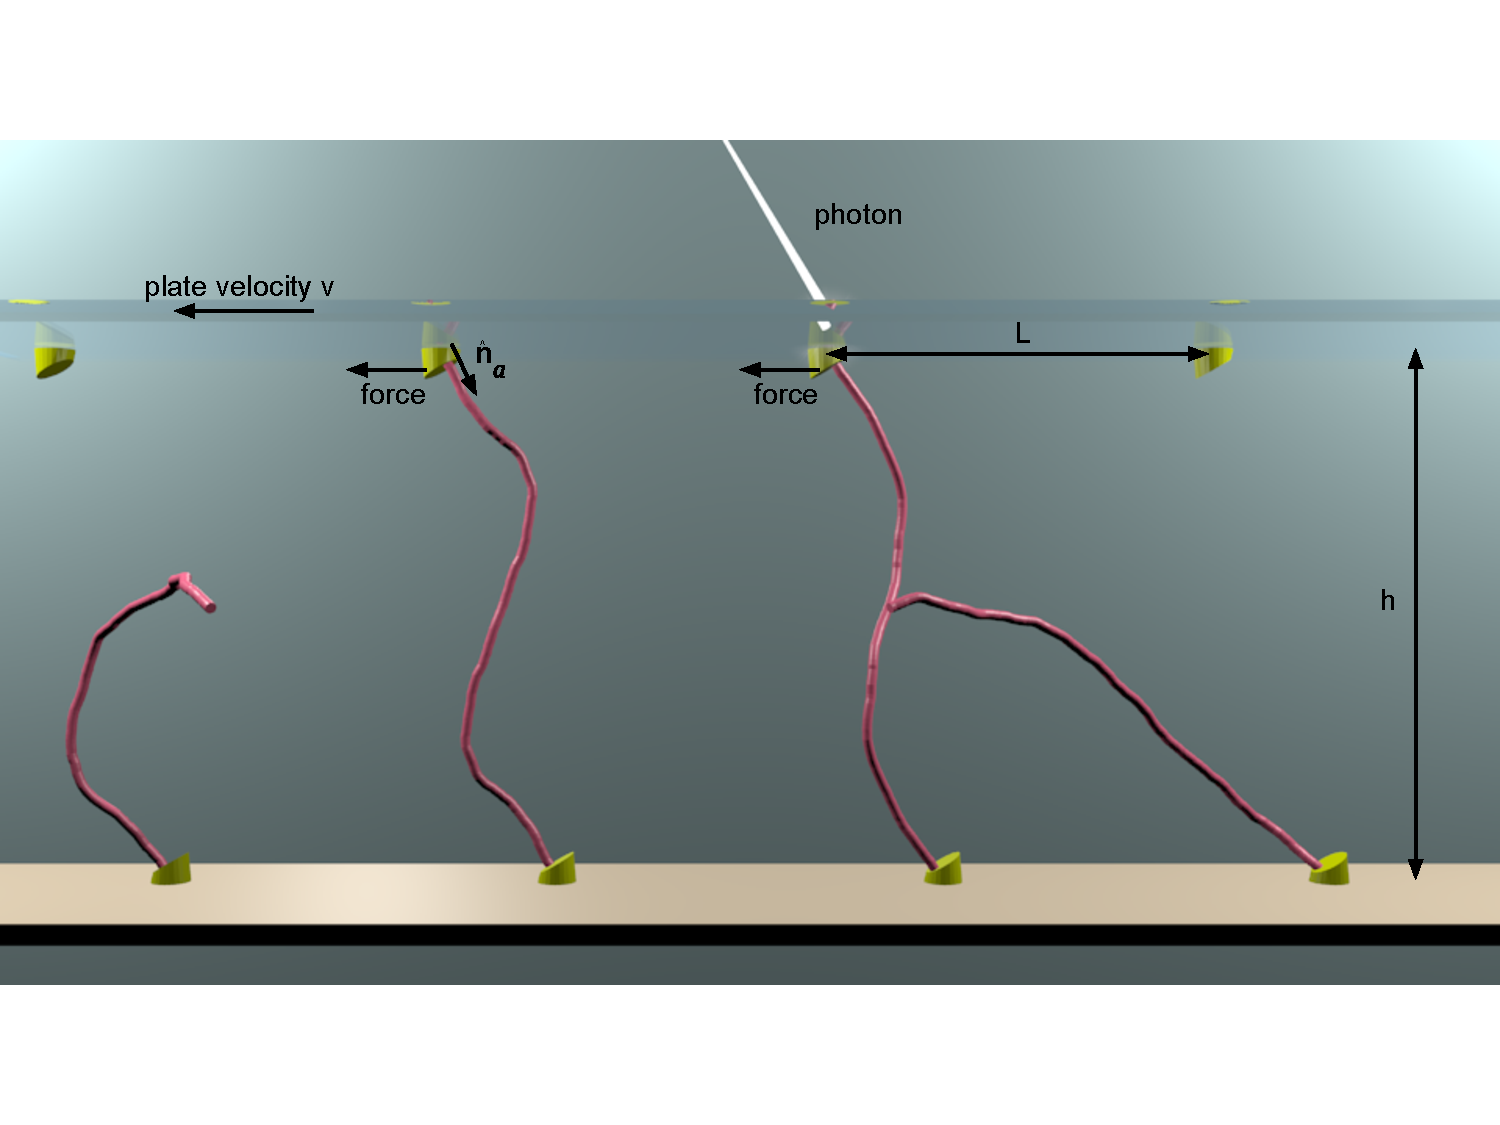
\includegraphics[width = \textwidth]{Fig1_label}
\caption{
(a) A schematic of the light energy to mechanical converter. A polymer
brush of semiflexible chains is put in contact
with a  plate a height $h$ above the base, containing an array of anisotropic binding sites with preferred binding direction ${\bf \hat n}_a$. Polymer ends are trapped by unlikely thermal fluctuations, applying a non-zero average force parallel to
the plate. Photodissociation of the polymer ends 
with the binding sites releases the chain end that will move until it finds
another site. The upper plate moves at a velocity $\rm v$, thereby generating
power. A single track is shown, and the separation between binding sites is $L$. The shape of the binding sites is meant only as a guide to the eye concerning the direction of ${\bf \hat n}_a$, and is not necessarily an indicator of the binding sites' physical structure.
}
\label{fig:device}
\end{center}
\end{figure*}

In most of the discussion below, the polymers can be considered to be separated
from each other by a sufficient distance so that we can ignore inter-chain interactions.
The absorption of light causing unbinding will happen asynchronously. The ends
tethered to the lower plates are at positions that are either random or
incommensurate with the binding sites of the upper plate. Altogether this means that
the motion of each polymer is uncorrelated with the others in the system.

The total effect of the forces acting on the plates can be used to perform
work against a force acting on the upper plate. Because we assume that
the number of polymers contributing is very large and are asynchronous, the net velocity of the
upper plate $v$ will be constant, as will be the net force acting on the plate.

In the following we will analyze the system and model it in different ways to 
better understand the power generation.


\section{Estimate of system parameters}
\label{sec:EOSP}

We will now make a crude estimate with realistic parameters of how well this device should work.
We envisage separate one dimensional tracks of the kind shown in Fig.
\ref{fig:device}. We do not enforce that the arrangement of binding sites need be a square two-dimensional array---the spacing between the tracks could indeed be much greater than the distances between polymers on a single track. This would have the effect of limiting polymers to a particular track of binding sites. In reality, it might prove more efficacious to manufacture a square array of polymers and binding sites
but we will allow two separate length scales in our analysis below.

We will assume a solar intensity of $I = 600 W/m^2$~\cite{SunLiu}, and an average photon energy of  $e = 2eV$~\cite{Gates}. We
will take the relaxation
time of a polymer to be $\tau = 10^{-7}s$, which corresponds roughly to a polymer size of $3nm$~\cite{degennes}.
The number of unbinding events, if every photon was
absorbed at a binding site, is $I/e \approx 2\times 10^{21}/(m^2 s)$. If the density of polymers is
$\sigma$, then for all of these events to be utilized requires $I/e = \sigma/\tau$, or
$\sigma = 2\times 10^{14}/m^2$, which is a separation of $1/\sqrt{\sigma} \approx 70 nm$.
The amount of energy per step that is gained by a photo-dissociation event is of
order $k_B T$. With such parameters, this is expected to yield an efficiency of
order $1\%$. However, as we will show below, longer relaxation times allow 
for more energy per step, and this requires a higher polymer density. However
the two dimensional density is limited by inter-chain interactions. In the case
considered here, this density could be increased roughly by three orders of
magnitude. However the
relaxation time for this system depends exponentially on the force generated, so 
a three order of magnitude increase in relaxation time
would only increase the efficiency by a factor of about $7$. Indeed, the
detailed analysis presented below suggests that with optimal conditions, the
efficiency of conversion is about $7\%$.
To increase the efficiency of solar conversion further might require stacking devices.

There are other means of increasing the solar conversion efficiency by first converting solar radiation to 
lower energy photons. For example, two methods for doing this are fluorescent down-conversion of solar
photons~\cite{Klampfatis}, or thermophotovoltaic down-conversion~\cite{Harder}.

Further speculation on device efficiency is premature as there will undoubtedly
be many unforeseen technical problems that will likely provide other obstacles
to increasing device efficiency. However an efficiency for direct
photo-mechanical conversion of about $7\%$ is still a useful amount of power
comparable to photovoltaic conversion with amorphous solar cells, and also because
power is lost in electro-mechanical conversion, which is not a problem with
direct mechanical energy conversion.

\section{Three dimensional model}
\label{sec:3Dmodel}

We start by simulating a three dimensional model of this system. There are two
components to the system, the polymer and the binding sites. The polymer chain
is modeled as having $N$ links of fixed length. Denote the coordinates of the $ith$ bead as $\br_i$. The elastic potential for the middle of the chain
for the $ith$ bead is
\begin{equation}
U_E(i) \equiv -\frac{C}{2}(|\br_{i+2}-\br_i|^2 + |\br_{i-2}-\br_i|^2)
\end{equation}
where $C$ is the stiffness constant.

The binding potential of the polymer has two components, an isotropic component
$U_i$ and directional component $U_d$. $U_i(r)$ is short range with a length
scale $r_s$ and scale $V_a$:
\begin{equation}
U_i(r) \equiv -V_a \exp\left(-\frac{A r^2}{r_s^2 - r^2}\right),
\label{eq:expU}
\end{equation}
where $A > 0$ is a parameter to adjust the shape of the potential. This binding potential is chosen for two reasons. First, $U_i(r)$ and all of its derivatives vanish as $r\rightarrow r_s$, thus all derivatives of these forces are continuous. Second, for small $A$, $U_i(r)$ rises quickly as $r\rightarrow r_s$, resulting in a large binding cross section. A plot of $U_i(r)$ for $A = 0.2$, $V_a = 60$, and $r_s = 1$ is shown in Fig. \ref{fig:expVplot}.

\begin{figure}[htp]
\begin{center}
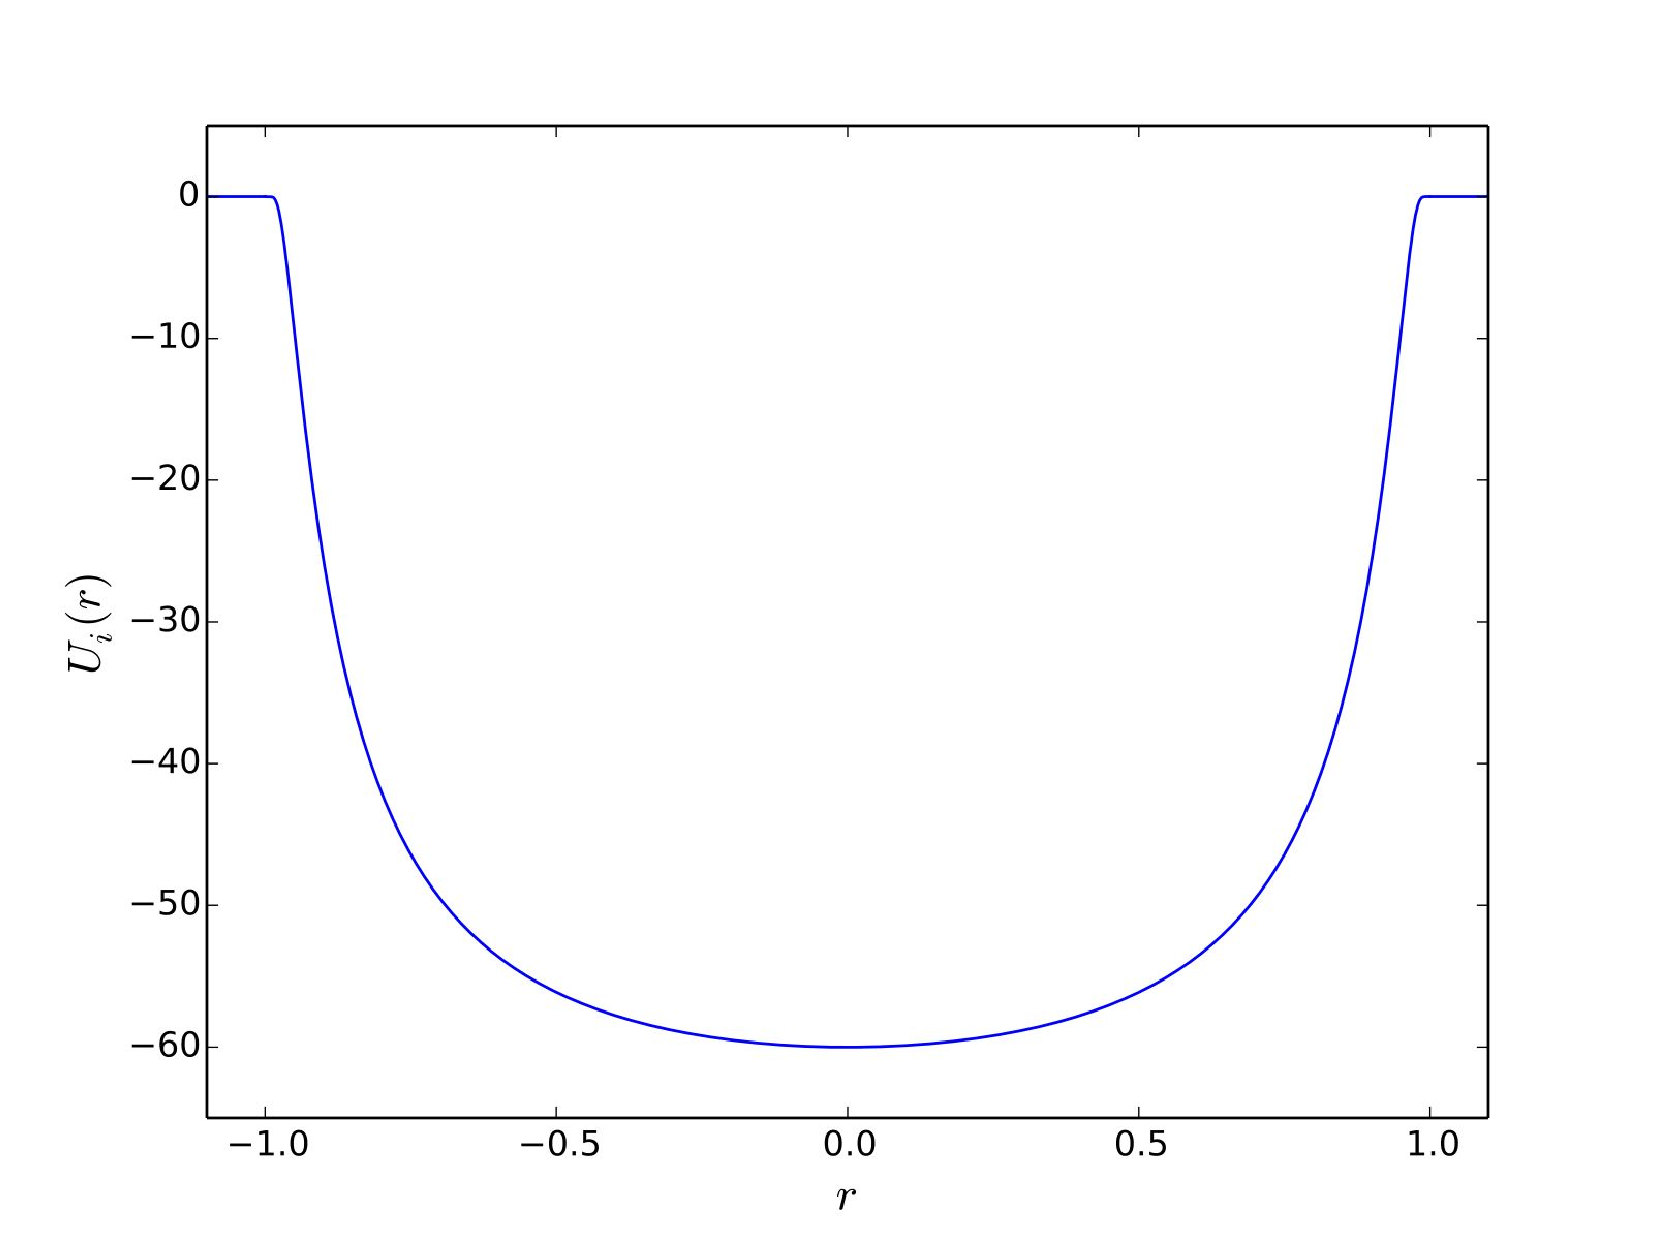
\includegraphics[width=\textwidth]{expVplot}
\caption{
A plot of the isotropic binding potential $U_i(r)$ vs. $r$, for $A=0.2$, potential well depth $V_a = 60$, and interaction length scale $r_s = 1$. 
}
\label{fig:expVplot}
\end{center}
\end{figure}

$U_d$ uses a direction $\nhat_a$ so that the difference
between the last two end beads $\delr = \br_1- \br_0$ will give a minimum in $U_d$
along that direction:
\begin{equation}
U_d(\br_0, \br_1) \equiv \left( \left| \frac{\delr}{|\delr|}-\nhat_a \right|^2 + 1 \right) U_i(r) .
\end{equation}

The end attached to the lower surface is always bound. The other end can bind to
a periodic linear array of binding sites equally spaced at a distance $L$.

There are two states that the system can be in, unbound, $0$, and bound, $1$. 
There are two parameters that control binding: the rate at which dissociation
occurs $c_1$, and the rate that dissociated ends can be rebound $c_0$.

The distance between the lower and upper surface is $h$ and their relative
velocity is $\rm v$.

The model was simulated with a Langevin equation, at finite temperature $T$.
Although inertial effects are typically small at these microscopic scales, it
was included for completeness. An algorithm was used that efficiently updates
this system with fixed link lengths~\cite{DeutschCerfFriction}.

In order to increase the rate of binding, we also restrict the vertical motion of the polymer to be between the two plates (i.e. $0\leq z\leq 1$ for $h=1$) and the lateral motion (perpendicular to $\bf{v}$) to a maximum distance of $h/2$ from the binding sites. These restrictions are not unrealistic--we expect motion of polymers in such a device to lie between the two solid plates, and lateral motion may be restricted by the polymer stiffness and/or interactions with other polymers.

The simulation was run to determine how the force and power 
generated are influenced by the plate velocity. Fig. \ref{fig:expVper} shows the
results of two simulations with different values of $c_0$ and $c_1$.
The parameters used were: $4$ links, $h=1$, spacing between binding sites $L = 2$, the direction of $\nhat_a$ 
is $\pi/4$, $V_a=60$, link length of $1$, particle mass of $1$, $C=0.5$,
$r_s = 1.0$, $A = 0.2$, and a coefficient of damping of $10$.

\begin{figure*}[htp]
\begin{center}
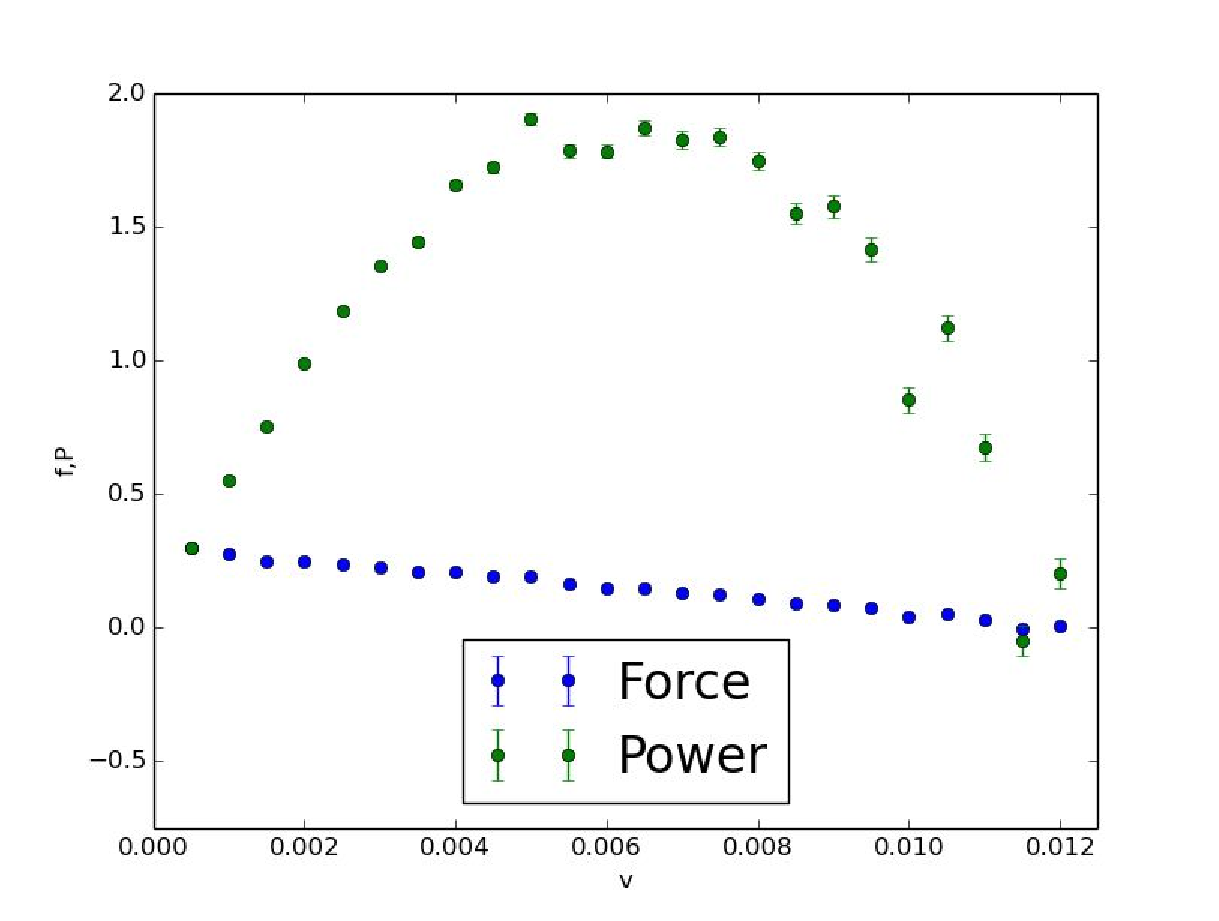
\includegraphics[width=4in]{0505per}\\
(a)\\
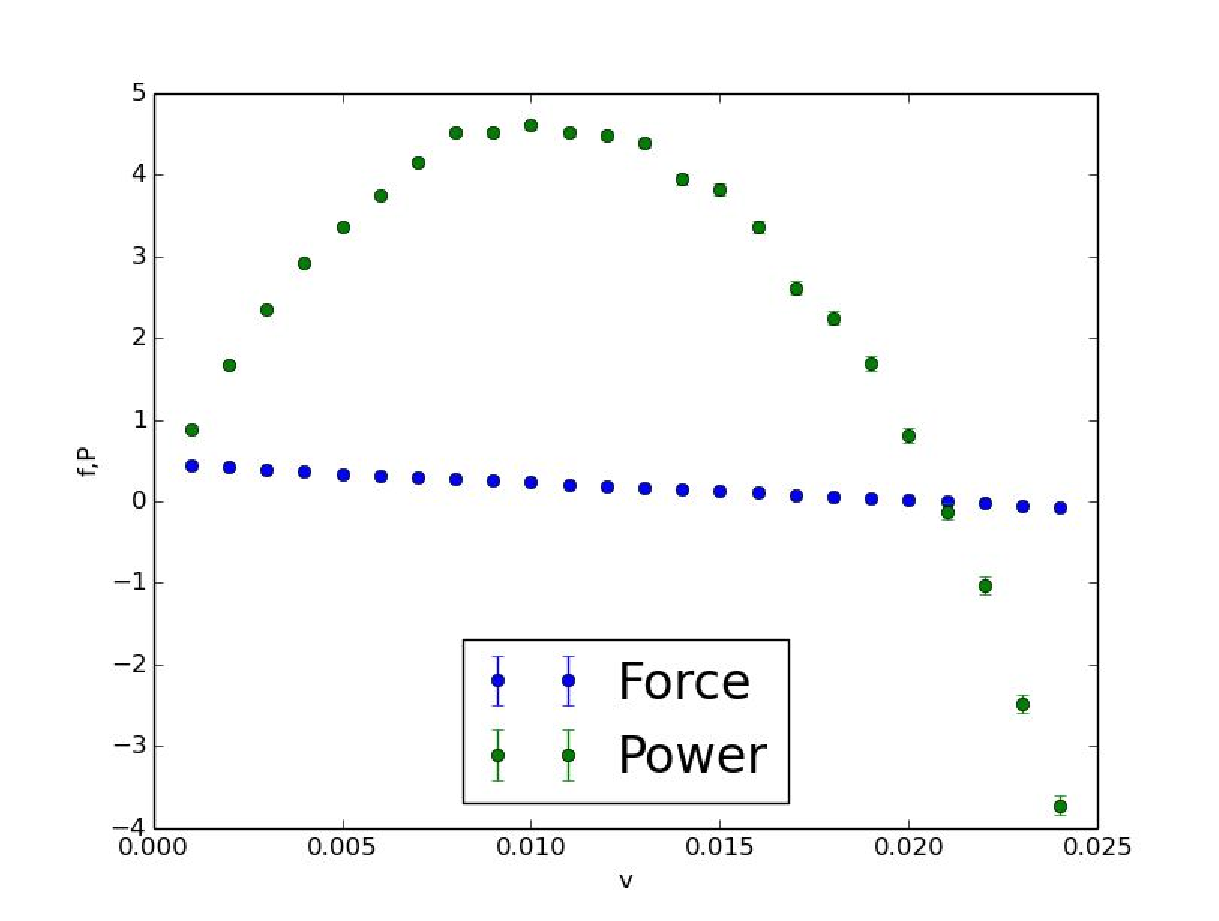
\includegraphics[width=4in]{4040per}\\
(b)
\caption{
The average force $f$ and the power $P=f {\rm v}$ measured as a function of the
relative velocity between the plates $\rm v$.  For clarity, the power is multiplied by $2000$. 
There were $4$ links, with a plate
separation of $h=1$, spacing between binding sites $L = 2$, the direction of $\nhat_a$ (that is, the binding angle) is
$\pi/4$, $V_a=60$, $A=0.2$, link length of $1$, stiffness constant $C=0.5$,
potential range $r_s = 1.0$, and a coefficient of damping of $10$. The coefficients of binding and unbinding, respectively, are (a) $c_0 = c_1 = 0.05$, and (b) $c_0 = c_1 = 0.4$.
}
\label{fig:expVper}
\end{center}
\end{figure*}

\begin{figure*}[htp]
\begin{center}
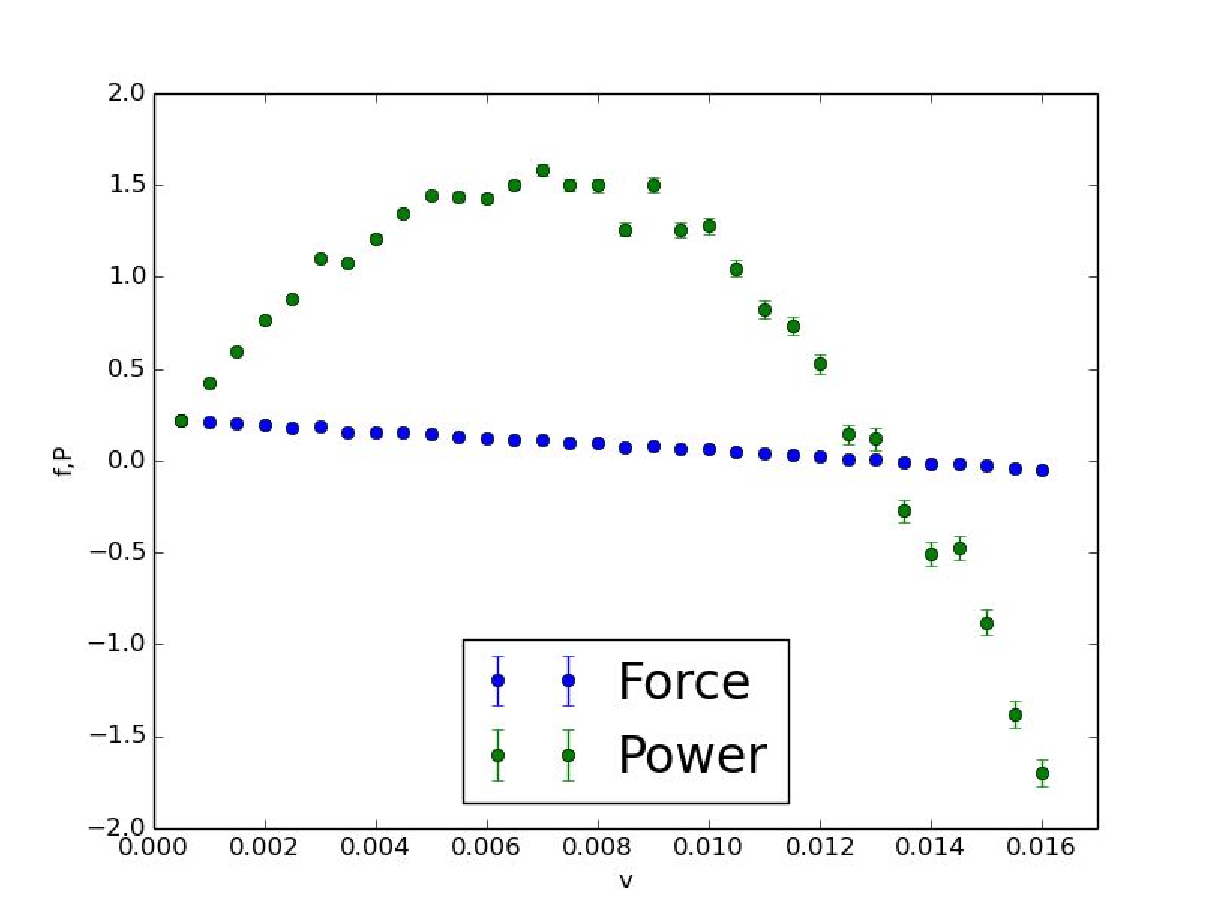
\includegraphics[width=4in]{0505rand}\\
(a)\\
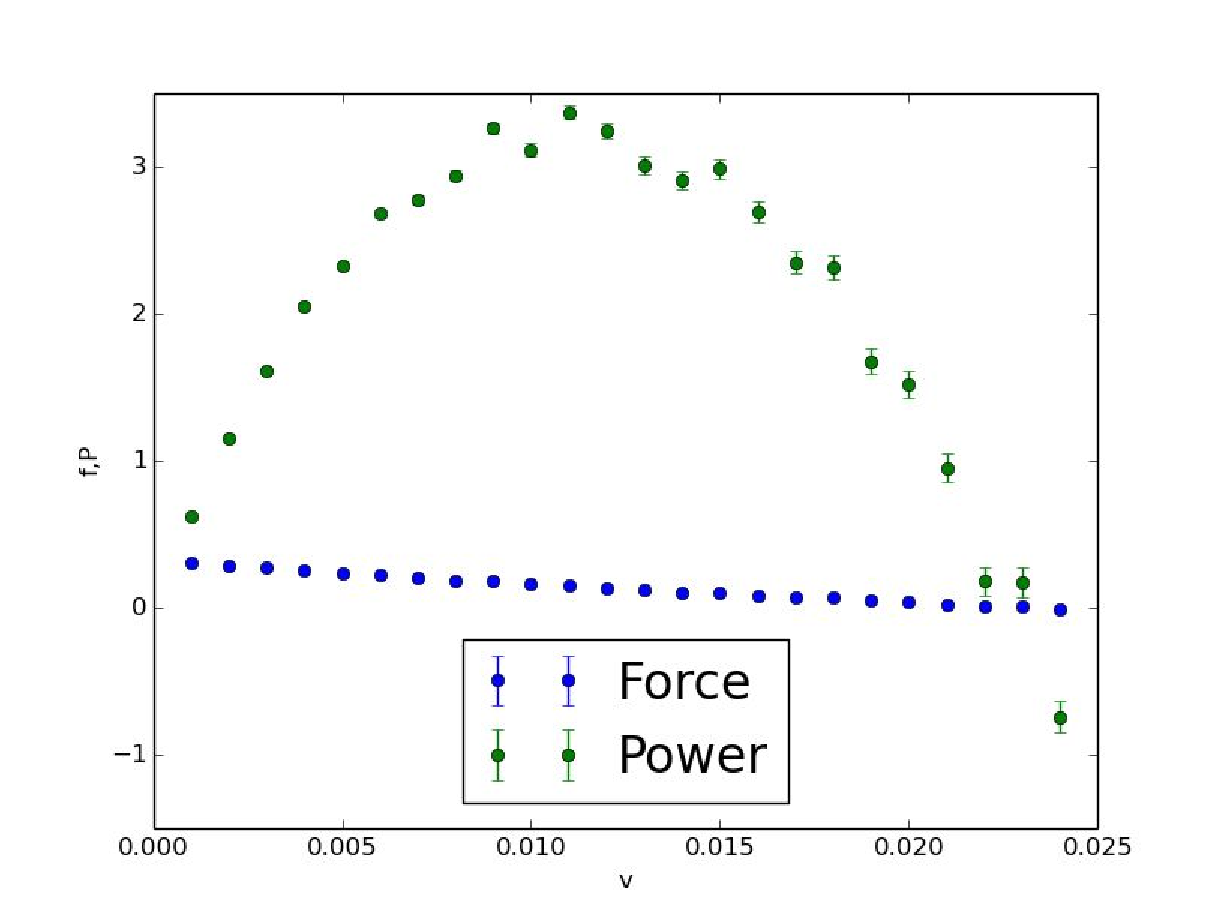
\includegraphics[width=4in]{4040rand}\\
(b)
\caption{
The average force $f$ and the power $P=f {\rm v}$ measured as a function of the relative velocity between the plates $\rm v$. The binding sites are placed randomly, with average binding site separation $\bar d = 2$ and minimum binding site separation $d_{min}=0.1$. Other than this, the same parameters and scaling are used as in Fig. \ref{fig:expVper}: (a) $c_0=c_1= 0.05$, and (b) $c_0=c_1= 0.4$.
}
\label{fig:expVrand}
\end{center}
\end{figure*}

The force generated is highest approaching zero velocity and decreases until it
becomes negative, at which point it is taking mechanical energy to move it at
such high speeds. Qualitatively, this is the point where frictional drag
dominates over photo-energy conversion.

Note that the highest force $f$, peak operating velocity, and power $P=f{\rm v}$ are all seen for $c_0 = c_1 = 0.4$. Higher maxima in the power are generally seen with increasing $c_0$ and $c_1$. However, this higher power is at the expense of efficiency, as higher
dissociation rates imply a higher photon flux.

It is also of interest to determine if this photomechanical effect persists if the binding sites are no longer periodic but instead are arranged at random. To investigate this situation, we place the binding sites so that the probability distribution of spacings, $d$, between binding sites followed Poisson statistics, that is $p_{spacing}(d) \propto \exp(-d/{\bar d})$. Here ${\bar d}$ is the average spacing between sites. However we also must introduce a lower cutoff, $d_{min}$, to prevent binding sites from overlapping so that when generating the next site's position, we reject spacings less than this cutoff. For our simulations, we set $\bar d = 2$ and $d_{min} = 0.1$. The purpose of this is to simulate possible experiments in which a rigidly periodic array of binding sites is impractical to construct.

Fig. \ref{fig:expVrand} shows the results of these simulations. The results are strikingly similar to those found with periodic sites. This shows that, at least for this parameter regime, the motor function of the device does not depend strongly on the regular placement of binding sites--an optimistic result from an experimental perspective.


\section{Steady State Probability Distribution}
\label{sec:SSPD}
To understand the above simulation in more detail requires a
better understanding of the mechanisms involved. There have been a very large
number of works on the theory of motor proteins~\cite{ReimannRev,BustamanteKellerOster}, and we will follow the two
state approach mentioned above of Prost {\em et. al.}~\cite{ProstPRL,JulicherRevModPhys}. 
The major difference is that they considered the two states to be periodic
potentials, whereas here we model the system to more closely mimic the
particular device we are investigating allowing the exploration
of force versus velocity. Hence instead of considering the
position of a particle moving between two periodic potentials, we consider
the unbound state to have a free end described as moving in a bound
potential around the tether point. Likewise, because of this tethering, the
bound state potential is not periodic but has a periodic component as we
will describe in detail below.
Here we consider the probability distribution for this system in steady
state, which is described by a Fokker Planck equation.

Initially to calculate the power that is produced, we will concentrate on the low velocity
limit, with the two plates moving so slowly that this motion does not affect
chain conformations appreciably. In this way, we can consider the average force
exerted between the plates by a polymer in steady state in the limit  ${\rm v}=0$ so that the
tether point is not moving. It is most convenient to let the point at which
the polymer is tethered to the bottom plate be a variable parameter $\br' = x' {\xhat}$.
With this point fixed, we consider the distribution of the other end of the
polymer $\br$.  We will assume that the internal dynamics of the chain
are much faster than the binding and unbinding rates, so that the only degrees
of freedom are $\br$, and if the polymer is bound, $i=0$ is unbound and $i=1$ is bound. Therefore the
probability distribution of the system can be described by a function
$P_i(\br;\br')$. The equations describing this are~\cite{ProstPRL}
\begin{subequations}
\label{eq:FP}
\begin{align}
\partial_t P_0(\br) = \nabla \cdot (\nabla - \bof_0)P_0(\br) - c_0 P_0(\br) + c_1 P_1(\br)\label{eq:FP0}\\
\partial_t P_1(\br) = \nabla \cdot (\nabla - \bof_1)P_1(\br) + c_0 P_0(\br) - c_1 P_1(\br)\label{eq:FP1}
\end{align}
\end{subequations}
where the last $\br'$ argument of $P$ has been left out for notational simplicity.
The units here absorb the diffusion coefficient $D$ together with the time, that
is $t$ as used here and below is really $D$ times the time. The force terms have 
absorbed a temperature factor $T$, that is $\bof_i$ is really the
force times $1/k_B T$.
Those forces $\bof_0$ and $\bof_1$ are the total forces acting on the upper end
of the chain. When the system is unbound, it is the force of a (possibly) nonlinear
spring 
\begin{equation}
\label{eq:unboundF}
\bof_0 = \bof_s(\br-\br'). 
\end{equation}
When the system is bound we have total force
is the sum of the spring force and a periodic force representing the binding
potential 
\begin{equation}
\label{eq:boundF}
\bof_1= \bof_s(\br-\br') + \bof_p(\br).
\end{equation}
These forces are assumed to be conservative, $\bof_s$ and $\bof_p$ are
derived from potentials that respectively are $V_s$ and $V_p$.

In steady state the left hand sides of Eqs. \ref{eq:FP}a-b are zero. We can
eliminate the last two terms on the right hand side to obtain
\begin{equation}
\label{eq:ohat1ohat2}
\Ohat_0 P_0 + \Ohat_1 P_1 = 0,
\end{equation}
where 
\begin{equation}
\label{eq:Ohatdefn}
\Ohat_i \equiv \nabla \cdot (\nabla - \bof_i), ~~~ i=0,1.
\end{equation}
We can now calculate the average force exerted by the two potentials, is zero. In steady
state, we multiply Eq. \ref{eq:ohat1ohat2} by $\br$ and integrate with respect to $x$, $y$
and $z$. Then using integration by parts, we have boundary terms at infinity.
Because we are assuming that the spring potential grows without bounds, this
confines $P_0$, and $P_1$, to a neighborhood around $\br'$, so that the boundary
terms vanish. We are then left with
\begin{equation}
\label{eq:P0plusP1}
\langle \bof\rangle = \int (\bof_0 P_0 + \bof_1 P_1) d^3\br = 0
\end{equation}
as is expected because $r$ is confined to a region of space so that the average
velocity, and hence average force, will be zero. 

We can also determine the total fraction of time spent in the bound or unbound
states in steady state. First, because the probability of being in any state is unity,
\begin{equation}
\int (P_0(\br) + P_1(\br)) d^3\br = 1 .
\end{equation}
Then by integrating Eq. \ref{eq:FP0} over all space, the derivative term
integrates to 0, giving
\begin{equation}
\int (-c_0 P_0(\br) + c_1 P_1(\br)) d^3\br = 0
\end{equation}
hence
\begin{equation}
\label{eq:norms}
\int P_0(\br) d^3\br = \frac{c_1}{c_0+c_1}, ~~~
\int P_1(\br) d^3\br = \frac{c_0}{c_0+c_1} .
\end{equation}


To obtain the power produced by this device, we are not interested in the total
force acting on the upper chain end because this includes the binding potential, but the
average force due to the spring acting on the lower plate $\langle f_s\rangle$. We would like
to calculate the work done in moving the lower point $\br'$ by one period of
$\bof_p$. After moving one period the system is statistically identical to its
starting point, and this method can therefore give the work done in moving $n$
such periods. Denoting the period of $\bof_p$ by $L$, we would like to calculate
\begin{align}
\label{eq:defnWL}
W_l &= \int_0^L \xhat\cdot \langle \bof_s\rangle dx' \nonumber\\
      &= \int_0^L \int \xhat\cdot \bof_s(\br,x'\xhat)(P_0(\br,x'\xhat)+P_1(\br,x'\xhat))d^3\br dx'
\end{align}
Using Eq. \ref{eq:unboundF} and \ref{eq:boundF}, this may be rewritten as
\begin{equation}
W_l = \int_0^L \int \xhat\cdot(\bof_0P_0(\br,x'\xhat)+(\bof_1 - \bof_p)P_1(\br,x'\xhat))d^3\br dx'
\end{equation} 
Eq. \ref{eq:P0plusP1} then yields
\begin{equation}
\label{eq:WL}
W_l = -\int_0^L \int \xhat\cdot \bof_p(\br)P_1(\br,x'\xhat)d^3\br dx' .
\end{equation}

In thermal equilibrium, where the transition rates $c_0$ and $c_1$ are both zero, 
we recover the Gibbs distribution. Let us assume, that the system starts, and
therefore remains in state $i=1$. Then
\begin{equation}
P_1(\br, \br') = \frac{e^{-V_1}}{Z}
\end{equation}
where the partition function 
\begin{equation}
Z(\br') = \int e^{-V_1} d^3\br 
\end{equation}
which will also have periodicity of $L$.
In this case $W_l$ can be easily calculated because $P_0 =0$ and $\bof_s = -\nabla
V_s(\br-\br') = \nabla'V_s(\br-\br')$. So 
\begin{eqnarray}
\label{eq:Weq0}
W_l &=& \int_0^L \int (\partial_{x'}V_s(\br,x'\xhat)) \frac{e^{-(V_s(\br-\xhat x')+V_p(\br))}}{Z(x')} d^3\br dx'\nonumber\\
    &=& -T (\log Z(L) - \log Z(0)) = 0
\end{eqnarray}
as it must be by the second law of thermodynamics.



\section{One dimensional solution}
\label{sec:1Dsol}
In order to investigate how the power conversion depends on the forces acting on
this system, it is important to simplify the three dimensional model to obtain
a minimal model that depends on far fewer parameters. Therefore we investigate
this model in one dimension.

A key point to understand is how asymmetry in the form of the force produces
power. With symmetric spring and binding potentials, it is easily seen by
symmetry that no net power can be produced from this system. We now ask how
asymmetry affects the results. We will see that even with a large asymmetry
in the spring potential, the work defined by Eq. \ref{eq:defnWL} is very small.
Simulations using Monte Carlo or Langevin equations are too noisy to provide
good estimates. We therefore instead use a more analytical approach.

The coupled Focker Planck Eqs. \ref{eq:FP} (a) and (b) can be solved to produce
an equation only involving one distribution function, $P_1$ in steady state.
Using the definitions in Eq. \ref{eq:Ohatdefn}, we can eliminate $P_0$.
\begin{equation}
(\Ohat_0\Ohat_1 - c_1 \Ohat_0 - c_0 \Ohat_1) P_1 = 0
\end{equation}
which is a fourth order equation in spatial variables.

Now we restrict the analysis to one dimension. In this case, $\Ohat_i = \px(\px-f_i)$
so we can integrate with respect to $x$. We note that because the spring
confines $P_1$ to a localized region, it will go to zero as
$x\rightarrow\pm\infty$. Therefore the integration constant must also be zero
\begin{equation}
\label{eq:1dDiffEq}
((\px-f_0)\px(\px-f_1) - c_1 (\px-f_0) - c_0 (\px-f_1)) P_1 = 0
\end{equation}
which is a third order linear differential equation.

Eq. \ref{eq:1dDiffEq} was solved by the shooting method~\cite{ShootingMethod}.
The boundary conditions were obtained by considering the system far from $x'$ where $P_0$ is very small. In that
domain, $f_p$ was artificially cutoff so that $f_0=f_1=f_s$. Because the
potential there is no longer changing between the two states, the solution is
that of a system in thermal equilibrium. The solutions were required to match to
these thermal solutions in this regime, far from $x'$.
The equation was solved with three different initial conditions. An appropriate
linear combination of these were constructed to match the boundary conditions as
just described.

The periodic binding potential that was used is
\begin{equation}
\label{eq:Vp}
V_p = A_1 \cos(x) - A_2 \sin(2 x) ~~.
\end{equation}

We first consider asymmetry in $V_s$ but with symmetric functions $V_p$, that
is, $A_2 =0$ in Eq. \ref{eq:Vp}.

\begin{equation}
\label{eq:nlfs}
V_s(x) \equiv \half k x^2 - \frac{a}{1+(b (x-d))^2} .
\end{equation}
The first term describes a linear spring with spring constant $k$, the second
adds an asymmetric dip. The parameters are chosen so that this dip is close
in potential to the one created predominantly by the linear term, $k=4$, $a=8$,
$b = 2$, and $d=2$. The function is plotted in Fig. \ref{fig:vs}.

\begin{figure}[htp]
\begin{center}
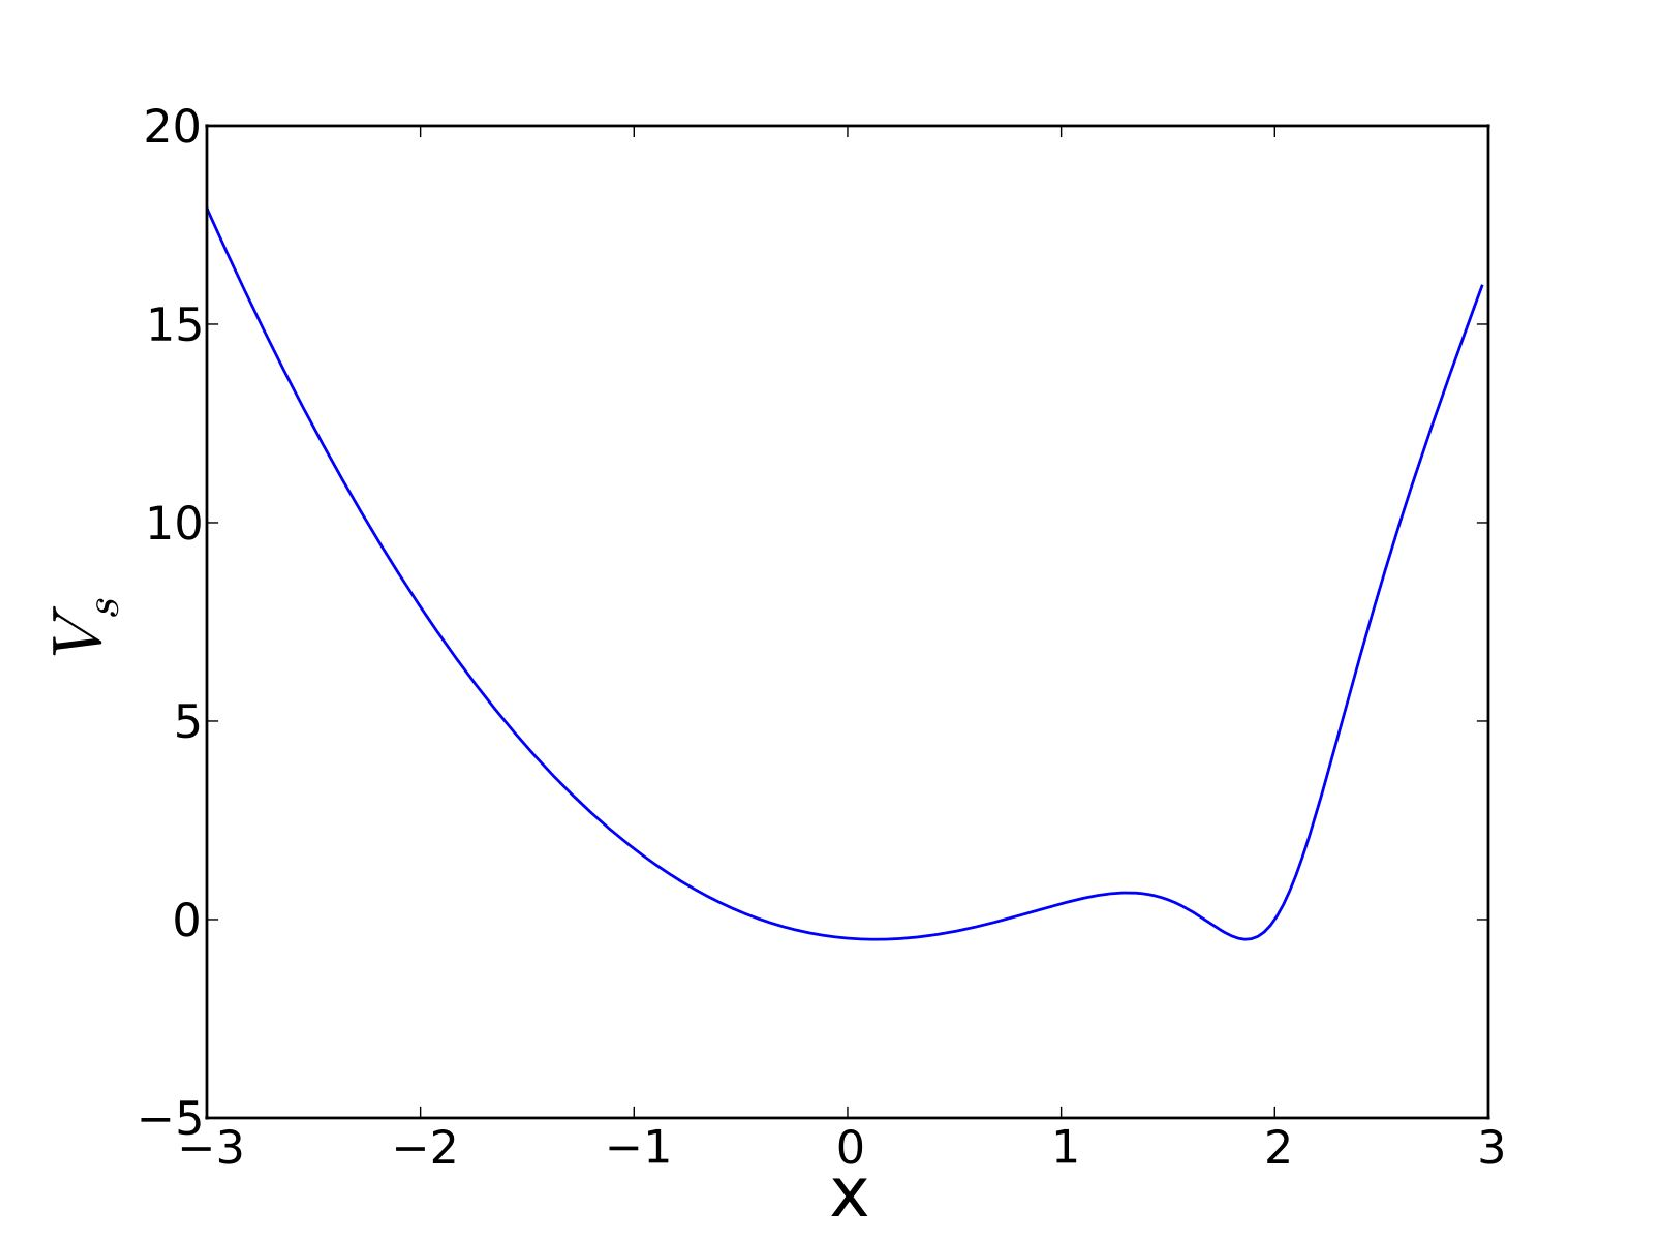
\includegraphics[width=\textwidth]{vs}
\caption{
An asymmetric spring potential used to tether the chain. It has a second dip at
approximately $x=2$
}
\label{fig:vs}
\end{center}
\end{figure}

Plots are shown in Fig. \ref{fig:Pnlspr} of $P_1(x)$ within a period for four values of $x'$: $-\pi,\ -\pi/2,\ 0,\ \pi/2$.

\begin{figure}[htp]
\begin{center}
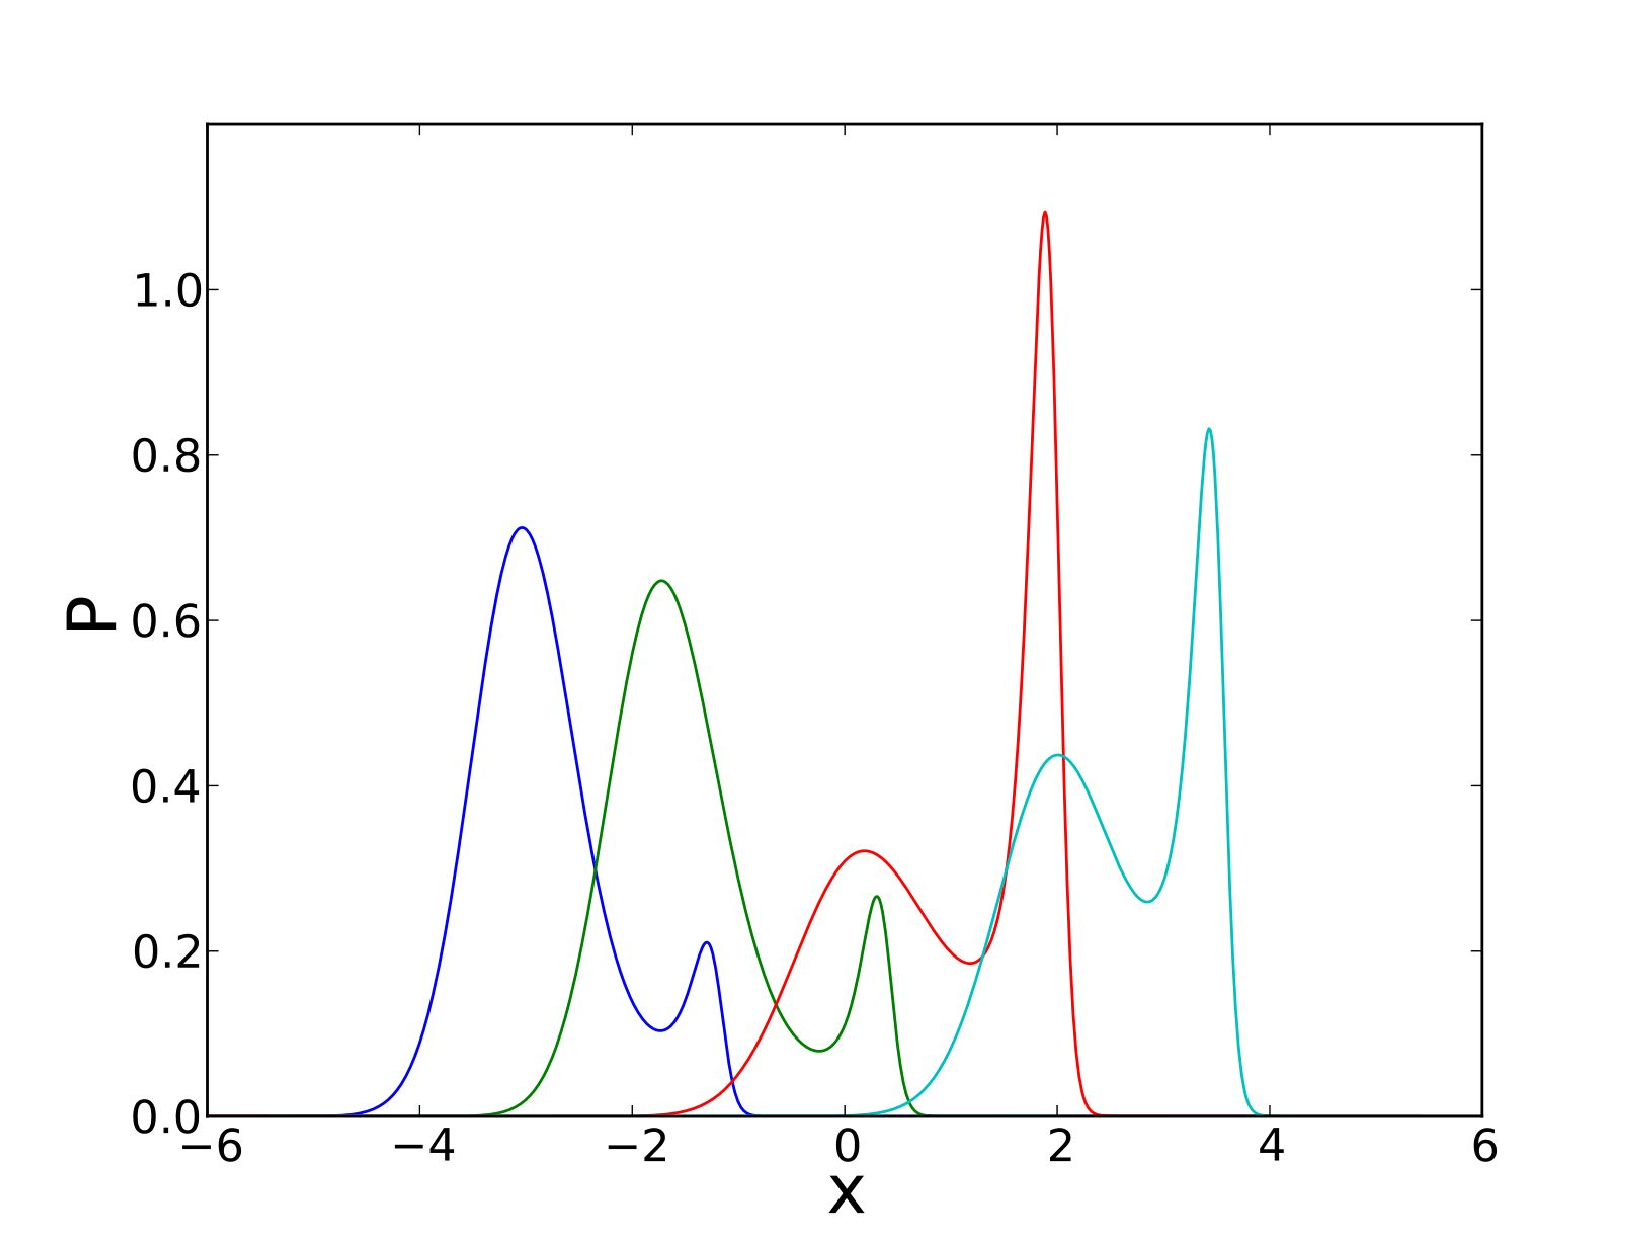
\includegraphics[width=\textwidth]{Pnl_spr}
\caption{
Plots of the probability distribution of $P_1$ as a function of position $x$
for $x' = -\pi,\ -\pi/2,\ 0$, and $\pi/2$ for the asymmetric spring model Eq. \ref{eq:nlfs}.
}
\label{fig:Pnlspr}
\end{center}
\end{figure}

By integrating using these distributions, Eq. \ref{eq:WL}, the work can be
obtained.  With $c_0 = 0.025$ and $c_1 = 0.05$ the work $W_L =   0.00080954$.
With the $c_i$'s $10$ times those values, 
$c_0 = 0.25$, and $c_1 = 0.5$, $W_L =  0.0025$. 

Now we consider the case of a linear spring so that the nonlinear parameter $a=0$
in Eq. \ref{eq:nlfs}. Instead we make the periodic potential asymmetric by
setting  $A_1 = A_2 =2$ in Eq. \ref{eq:Vp}, still with
$c_0 = 0.25$, and $c_1 = 0.5$. 
Fig. \ref{fig:Pasvp} plots $P_1(x)$ within a period for the same four values of $x'$ in Fig. \ref{fig:Pnlspr}.

\begin{figure}[htp]
\begin{center}
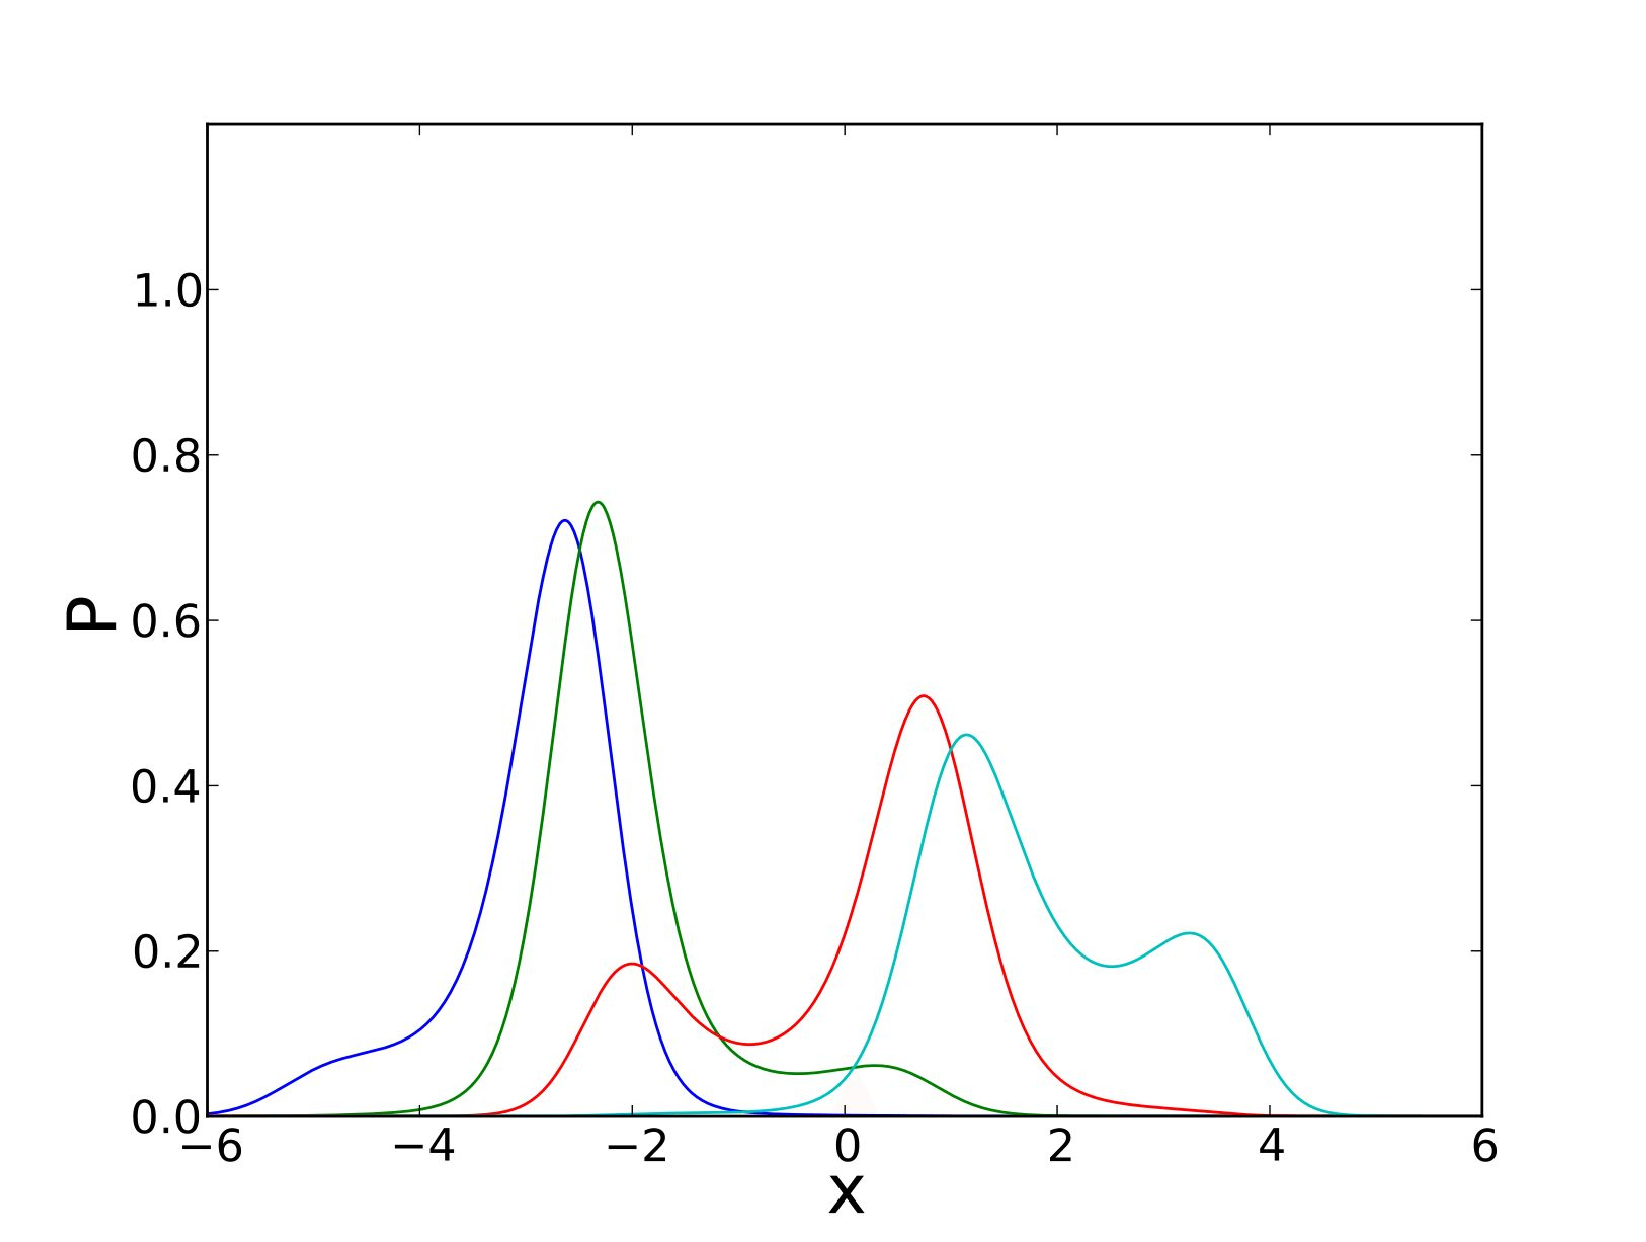
\includegraphics[width=\textwidth]{Pasvp}
\caption{
Plots of the probability distribution of $P_1$ as a function of position $x$
for the values of $x'$ shown in Fig. \ref{fig:Pnlspr}, but for an asymmetric periodic potential and a linear
spring.
}
\label{fig:Pasvp}
\end{center}
\end{figure}

In this case, the work $W_L = -0.1596$.

What the numerical results have shown is that asymmetry in the spring potential
is quite ineffective at producing work, whereas asymmetry in the periodic
binding potential is much more effective. We shall use this result below and concentrate
on systems with symmetric spring potentials, but asymmetric binding potentials.

\section{Unbound Equilibration Model}
\label{sec:UEM}
It is worthwhile to
understand in more detail what constrains the maximum force of photo-mechanical conversion by
tuning the potentials employed and the binding rate, and to ask how the design will depend on 
the flux of photons. We are limited in our choice of the potentials $V_0$ and
$V_1$ that both must be bounded. In this system, the unbound potential is not periodic which
limits the amount of power that can be generated. In cases considered earlier~\cite{ProstPRL}, where both
potentials are periodic, it is possible to get much more efficient motion by
alternating between states with different potential maxima. However this is not
relevant to our system.

To understand this better, it is useful to examine a limit where we can treat
the system analytically. We therefore examine the case where the 
binding rate of an unbound chain is sufficiently small, so that we can regard it in thermal
equilibrium. 

The model is illustrated in Fig. \ref{fig:1dpot}. We take the unbound potential
to be that of a linear spring below a cutoff
\begin{equation}
\label{eq:v0cutoff}
V_s = V_0 =\begin{cases}
k (x - x')^2/2 , & \text{if $-l_c < (x-x')< l_c$}.\\
\infty, & \text{otherwise}.
\end{cases}
\end{equation}
we choose the spring coefficient $k$ such that
$l_c \exp(-k l_c^2/2) \ll 1$.  Below, we will take $l_c = L/2$ or $\infty$.

The periodic potential $V_p$ is taken to be localized at periodic points (with
a separation of $L$) that rapidly vary from a large maximum $V_{max}$ to a
minimum $V_{min}$, as shown. We take the region over which this happens to be
negligibly small compared to other length scales in the problem.\\
\vfill

\begin{figure}[htp]
\begin{center}
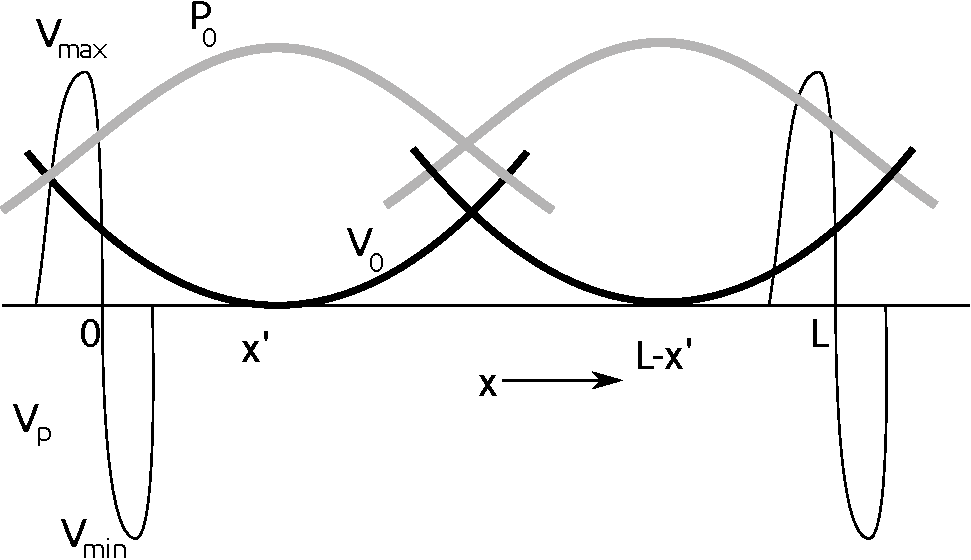
\includegraphics[width=\textwidth]{1dpot}
\caption{
Illustration of the kind of potentials employed in the Unbound Equilibration
Model. The periodic potential $V_p$ is nonzero only on small regions on the
x-axis. It shows a large peak of height $V_{max}$ and large negative dip
$V_{min}$. There spring potential $V_0$ is parabolic, except that it has a
cutoff where it becomes infinite when stretched by more than $l_c$. The
corresponding probability distribution $P_0$ (grey curve) is assumed to have relaxed to
equilibrium. The spring potential is shown at two different position, when it
is centered at $x'$ and $L-x'$.
}
\label{fig:1dpot}
\end{center}
\end{figure}

In the following, we present a new analytical method that allows us to systematically solve for the behavior of this kind of nonequilibrium system in the limit of large activation barriers. To understand how equilibration can occur in this model, we can rewrite 
Eqs. \ref{eq:FP} in the steady state limit
%\begin{subequations}
%\label{eq:SFP}
%\begin{align}
%\nabla \cdot (\nabla - \bof_0)P_0(\br) - c_0 P_0(\br) = -c_1 P_1(\br)\label{eq:SFP0}\\
%\nabla \cdot (\nabla - \bof_1)P_1(\br) - c_1 P_1(\br) = -c_0 P_0(\br) \label{eq:SFP1}
%\end{align}
%\end{subequations}
%
%%%%
%%%%JOSH: We could shorten this a bit:
%%%%
\begin{equation}
\label{eq:SFP}
\nabla \cdot (\nabla - \bof_i)P_i(\br) - c_i P_i(\br) = -c_{1-i} P_{1-i}(\br), ~~ i=0,1
\end{equation}

Although this is time independent, we consider the related time dependent equations for
variables $\tilde{P}_i(\br, t)$
%%%%JOSH: And this:
%\begin{subequations}
%\label{eq:LFP}
%\begin{align}
% \partial_t \tilde{P}_0(\br)-\nabla \cdot (\nabla - \bof_0)\tilde{P}_0(\br)  = 0 \label{eq:LFP0}\\
% \partial_t  \tilde{P}_1(\br)-\nabla \cdot (\nabla - \bof_1)\tilde{P}_1(\br)  = 0 \label{eq:LFP1}
%\end{align}
%\end{subequations}
\begin{equation}
\label{eq:LFP}
 \partial_t \tilde{P}_i(\br)-\nabla \cdot (\nabla - \bof_i)\tilde{P}_i(\br)  = 0, ~~ i = 0,1
\end{equation}
where $P_i$, $i=0,1$, is the Laplace transform of $\tilde{P}_i$, $P_i(s) = \mathcal{L} \{\tilde{P}_i\}$, where the conjugate variable
for $i=0,1$ are $s =c_0$ and $s = c_1$, respectively. Taking the Laplace transform of both sides of Eqns. \ref{eq:LFP} yields Eqns. \ref{eq:SFP}, with the initial conditions 
%%%%JOSH: And this:
%\begin{subequations}
%\label{eq:IFP}
%\begin{align}
%\tilde{P}_0(\br,t=0) = c_1 P_1(\br,s=c_1) \label{eq:IFP0}\\
%\tilde{P}_1(\br,t=0) = c_0 P_0(\br,s=c_0) \label{eq:IFP1}
%\end{align}
%\end{subequations}
%%%%JOSH: the same way:
\begin{equation}
\label{eq:IFP}
\tilde{P}_{i}(\br,t=0) = c_{1-i} P_{1-i}(\br,s=c_{1-i}) , ~~ i=0,1
\end{equation}

These equations have a direct physical interpretation. The left hand sides in
Eqs. \ref{eq:LFP} are those of particles diffusing in potentials, but with
conservation of particles. For long enough times, independent of initial
conditions, the solution to these equations will go to thermal equilibrium given
by the Gibbs distribution. 
%%%%% JOSH: replace: 
%Eq. \ref{eq:LFP0} describes diffusion in a quadratic potential. We require that
%with
Eq. \ref{eq:LFP}, $i=0$,  describes diffusion in a quadratic potential. We require that
we are probing this at long enough times $t$, so that it will have nearly
reached this equilibrium state. Call this longest relaxation time $\tau_0$.
The solution to the diffusion equation $\tilde{P}_0(\br,t)$ for either $i=0,1$ in Eq.
\ref{eq:LFP}, can be written as a sum over spatial
eigenfunctions, $\phi_n(\br)$ that decay at different rates $\lambda_n$,
(arranged to be monotonically increasing):
\begin{equation}
\label{eq:phiexpansion1}
\tilde{P}_0(\br,t) = \sum_{n=0}^\infty \phi_n(\br) \exp(-\lambda_n t), 
\end{equation}
of which the smallest $\lambda$, $\lambda_0 = 0$, corresponds to the equilibrium state. The relaxation
time is $\tau_0 = 1/\lambda_1$, thus the Laplace
transformed variable $P_0$ can be written
\begin{equation}
\label{eq:phiexpansion2}
P_0(\br,s) = \sum_{n=0}^\infty \phi_n(\br) \frac{1}{s+\lambda_n} .
\end{equation}
If the $n=0$ term is to dominate, we therefore require $s = c_0 \ll 1/\tau_0$.
The physical interpretation of this condition is that binding typically occurs only after
many relaxation times of the unbound end.

$P_0(\br, s=c_0)$ will be dominated by the first term in Eq. \ref{eq:phiexpansion2}
and therefore proportional to the eigenfunction $\phi_0(\br)$ which is
the equilibrium distribution and is $\propto \exp(-V_0)$.
An important simplifying point in the above approach is that the precise form of
the initial condition Eq. \ref{eq:IFP}, $i=0$, is not important, but because of
particle conservation, only the total area under $P_1$ affects the result.


Now we consider the solution for $P_1$. If we consider unbinding times much
longer than the relaxation time in the bound state, we also arrive at thermal
equilibrium, which was shown by Eq. \ref{eq:Weq0} to lead to no work being performed. Instead
we will consider situations where there are very long lived metastable states.
%%%%JOSH: Replace
%In Fig. \ref{fig:1dpot}, the potential seen by a particle in Eq. \ref{eq:LFP1}
%with
In Fig. \ref{fig:1dpot}, the potential seen by a particle in Eq. \ref{eq:LFP}, $i=1$,
is $V_1 = V_0 + V_p$. If a particle starts between $0$ and $L$, it will remain
trapped in that region for a Kramer's time which (ignoring algebraic pre-factors)
depends on $x'$, but has a minimum value of $\tau_m \propto \exp(V_{max})$. By
choosing large enough $V_{max}$ this can be made arbitrarily long. 

A particle in such a metastable state will relax to a metastable equilibrium,
obeying Eq. \ref{eq:phiexpansion1} that will eventually fail for times $t >
\tau_m$. In this expansion, the longest relaxation time to this metastable state
$\tau_1 = 1/\lambda_1$,
will be taken to be much smaller than $\tau_m$. Thus the above argument on the
range of $c_0$ can be used {\em mutatis mutandis} to restrict
the unbinding rate to $1/\tau_m \ll c_1 \ll 1/\tau_1.$

%%%%JOSH: Replace
%In this regime we can understand the solution to  Eqs. \ref{eq:LFP1} and \ref{eq:IFP1} 
%with
In this regime we can understand the solution to  Eqs. \ref{eq:LFP} and \ref{eq:IFP}, $i=1$ 
by considering the corresponding Green's function $\tilde{G}(\br,t;\br_0)$. We replace the initial
condition Eq. \ref{eq:IFP}, $i=1$, by 
\begin{equation}
\label{eq:GIFP} 
\tilde{G}_1(\br,t=0;\br_0) = \delta(\br-\br_0) . 
\end{equation}

We can then obtain $\tilde{P}_1$ from the Green's function from
\begin{equation}
\label{eq:P1intGP0}
\tilde{P}_1(\br,t) = \int \tilde{G}_1(\br,t;\br_0) c_0 P_0(\br_0, s = c_0) d^3\br_0 .
\end{equation}

For a wide range of times, and regions of $\br'$, $\tilde{G}_1$ will approach the same
metastable state. A particle starting at any point within a certain region will
end up stuck in the same state and hence approach the same metastable equilibrium. 
Confining our attention to the one dimension model of Fig.
\ref{fig:1dpot}, for $0 < x_0 < L/2$ the solution will be strongly localized at
the minimum $x=0$. For $L/2 < x_0 < L$ the effects of $V_p$ are negligible
and $\tilde{P}_1(x) \propto \exp(-V_0)$. This is because the potential $V_0$ 
in Eq. \ref{eq:v0cutoff} is cutoff which does not allow the particle to visit
the $x=0$ region. Hence the effect of $V_p$ is only seen close to $x=L$ where
it provides a strong repulsion, but over a negligibly small region of $x$.
For $-L/2 < x_0 < 0$, $V_p$ also does not contribute.
For $L < x_0 < 3L/2$ the solution will be strongly localized at
the minimum at $x=L$. Because of particle conservation, the area under
$\tilde{G}_1$ is always unity.

A physical interpretation of the above equations in terms of a one dimensional one particle system 
can now be made using the Laplace transformed
variables and the metastable limit considered above is now apparent.
In the unbound state, the
particle reaches thermal equilibrium relaxing to the Gibbs
distribution, $P_0 \propto \exp(-V_0)$. Then the periodic potential $V_p$ is suddenly
added in. The position at the time of switching is labeled $x_0$. Depending
on which interval $x_0$ is in, $x$ will equilibrate to the corresponding
metastable equilibrium with $P_1 \propto \exp(-V_1)$ and is completely confined to
that interval. The relative probabilities
being in one of the three above regions is obtained by the area under $P_0$ for
that interval.

Now that we know how to determine $P_0$ and $P_1$, we would like to calculate the
work $W_l$ given by Eq. \ref{eq:defnWL}. Because of the symmetric form assumed
for $f_s$, the $f_0 P_0$ term in the integrand gives zero contribution and we
are left with
\begin{equation}
\label{eq:symWL1d}
W_l = \int_0^L \int_{-\infty}^\infty  f_0(x-x') P_1(x,x')dx dx'
\end{equation}
and consider first how to calculate the inner integral
\begin{equation}
\label{eq:F1d}
f_l(x') \equiv \int_{-\infty}^\infty f_0(x-x') P_1(x,x')dx 
\end{equation}
where $x'$ is the position of the tethered end.  Eq. \ref{eq:v0cutoff} gives $f_0(x) = -kx$ for $|x|<L/2$.

Using the prescription we have found for $P_1(x,x')$, which is simplified by the above physical interpretation, we can partition this integral
into the different $x$-intervals of metastability: $I_- \equiv[-L/2,0]$, $I_0 \equiv [0,L]$, and $I_+ \equiv [L,3L/2]$.
The value of $P_1(x,x')$ depends on the probability of initially being trapped in
one of those three intervals. Because of the cutoff we have imposed on $V_0$,
only two intervals need be considered for a given value of $x'$. For $0 < x' < L/2$, only intervals $I_-$ and
$I_0$ occur.  The probability that $x \in I_-$ given $x'$ is
\begin{equation}
E(x') \equiv P(x \in I_-| x') = \int_{-\infty}^0 p_0(x-x') dx  = \int_{x'}^\infty p_0(x) dx
\end{equation}
and the probability that $x \in I_0$ is $P(x \in I_0|x') = 1-E(x')$.
Here $p_0(x)$ is proportional to $P_0(x)$ but normalized to unity, to simplify
the presentation.
We can obtain the values for $L/2 < x' < L$ by symmetry, so that $P(x \in I_+| x') = E(L-x')$ and
$P(x \in I_0|x') = 1-E(L-x')$.  In the limit considered here, the effects of the cutoff in the potential will have a negligible effect. For this reason, $p_0(x)$ will be a normal distribution and thus $E(x')$ is simply related to the complementary
error function, $E(x') = \frac{1}{2}erfc(\sqrt{k}x')$. 

At this point, it is possible to evaluate Eq. \ref{eq:symWL1d} directly. However, for simplicity, we take a more intuitive approach: there is a symmetry in many of the quantities considered, as shown in Fig. \ref{fig:1dpot} where the
potential $V_0$  and corresponding probability distribution $p_0$ is for the tethering point at
$x'$ and at $L-x'$. Therefore it is convenient to consider the quantity $f_{l/2}(x')\equiv f_l(x') + f_l(L-x')$. 

Additionally, by equation \ref{eq:F1d}, $f_l$ can be thought of as an expectation value, or weighted average. Any expectation value can be expressed as a weighted sum of expectation values broken down by region.
%%%%
%%%%JOSH: We can probably leave all this out:
%%%%
%With this in mind, $f_{l/2}$ can be written as
%\begin{align}
%\label{eq:flplusfl}
%f_{l/2}(x')=-\frac{k c_0}{c_0+c_1} &\left[-E(x')\langle x \rangle' +  E(x') x' \right.\nonumber\\
%&\left. -(1-E(x'))x' + (1-E(x'))\langle x\rangle''\right]
%\end{align}
%where
%\begin{equation}
%\langle x \rangle' \equiv -\frac{\int_{-\infty}^0 (x-x')p_0(x-x')dx}{\int_{-\infty}^0 p_0(x-x')dx} 
%= \frac{\int_{x'}^\infty x p_0(x)dx}{E(x')}
%\end{equation}
%and
%\begin{equation}
%\langle x \rangle'' \equiv -\frac{\int_{-\infty}^0 (x+x')p_0(x+x')dx}{\int_{-\infty}^0 p_0(x+x')dx} 
%= \frac{-E(x')}{1-E(x')} \langle x \rangle' .
%\end{equation}
%
%The four terms in Eq. \ref{eq:flplusfl} correspond to contributions from respectively regions $I_-$, $I_+$ , $I_0$, and
%$I_0$. The first and third term are contributions from $f_l(x')$ and the others
%are from $f_l(L-x')$. The factors involving $c$ give the correct normalization
%according to Eq. \ref{eq:norms}. Combining the above equations, 
%%%%%
%%%%%JOSH: Now we can continue saying:
%%%%
This yields
%%%%JOSH: and continuing as before:
\begin{equation}
W_l = \frac{k c_0}{c_0+c_1} \int_0^{L/2} 2 E(x')(\langle x\rangle' - x') + x' dx' .
\end{equation}


In the limit of large $L$, which we are considering by virtue of the condition
on the cutoff in $V_0$ imposed by Eq. \ref{eq:v0cutoff}, the integrand
simplifies because $\langle x\rangle'$ becomes exponentially close to $x'$, and
the only term remaining is $x'$. Thus for large $L$, $W_l = (c_0/(c_0+c_1))k L^2/8$.
The factors involving the $c$'s represent the fraction of time spent in the
bound configuration. The last term increases quadratically with $L$. This result
is misleading if not taken with the appropriate limits that have been assumed in
its derivation. The factor $(c_0/(c_0+c_1))$ is very close to unity as we are
assuming that the relaxation time in the unbound state is much faster than in
the bound state, hence $c_0 \gg c_1$. However the work $W_L$ to move a distance
$L$ was assumed to be in the adiabatic limit, and here the time scales
associated with bound state relaxation are exponentially long. This is because
to reach this metastable equilibrium the particle has to hop over barriers of
size $V_0(x')$, see Fig. \ref{fig:1dpot}. Hence the  longest relaxation time for this is
at $x'=L/2$ and is of order $\exp(kL^2/4)$. Note that this does not contradict
our assumption that we are still in a region of metastability, which requires
times much less than $\exp(V_{max})$. But for this to work, we require that $V_{max} \gg V_0(L/2)$.

Now we consider the case where the spring length cutoff $l_c \rightarrow \infty$. The
disadvantage of this is that the chain end can, in principle, hop over many
barriers ending up arbitrarily far from the tether point, and that these hopping
times should be included in the above analysis. However, the probability of such
a hop becomes negligible when the probability of finding the chain end there is small. Hence we
still have a clear separation of time scales between metastable states as
discussed above, and fully equilibrated system, which requires surmounting the
energy barrier $V_{max}$. In this case, we can therefore assume that when the
chain end $x'$ is between $nL$ and $(n+1)L$, it will strongly localized at $x' = nL$. 
Therefore 
\begin{equation}
\label{eq:inflcfl}
f_l(x') = -k \sum_{n=-\infty}^\infty \Delta_n(x') (nL-x')
\end{equation}
where $\Delta_n(x')$ is the probability of initially finding the chain end
between $nL$ and $(n+1)L$, 
\begin{equation}
\Delta_n(x') = E(nL-x')-E((n+1)L-x').
\end{equation}
It is easily seen that $\Delta_{-n}(L-x') = \Delta_n(x')$. Using this and Eq. \ref{eq:inflcfl}
\begin{equation}
f_l(L-x') = -f_l(x') +kL \sum_{n=-\infty}^\infty \Delta_n(x') =  -f_l(x') +kL  .
\end{equation}
To obtain the work, we follow the same procedure as above and consider $f_l(x') + f_l(L-x')$, which
here is just $kL$. Therefore in this case,
\begin{equation}
W_l = \frac{c_0}{c_0+c_1} \frac{k L^2}{2}.
\end{equation}
This is an exact value for this model, for all $k$ and $L$, given that we are in a region
of strong metastability.

\subsection{Efficiency in large power stroke limit}
\label{sec:EILPSL}
We now are in a position to answer a central question about the performance of
this kind of device: is the efficiency limited by the small value of $k_B T$
compared to photon energies? We have seen from the above analysis that it is
possible to get arbitrarily large forces developing at the expense of
exponentially slow operation. However this is in the limit of infinitesimal
plate velocity $\rm v$. In contrast, the power obtained is instead average
force times this, $\langle f\rangle {\rm v}$ and we would like to operate the
device at the velocity of maximum power, which necessitates the operation of it
far from equilibrium, because compensating the increase in $\rm v$ is a
decrease in $\langle f\rangle$ due to dissipation. It could be that the optimum velocity of operation
decreases very quickly with $k L^2/2$ meaning that the device becomes
increasingly inefficient as the spring constant $k$ is increased. This would
make it impossible to harvest more than of order $k_B T$ energy per cycle.

The efficiency is defined as the ratio of the amount of power produced to the
amount of power put in. The amount of energy needed to dissociate a polymer end
from a binding site is $V_{min}$. Binding to $V_{min}$ must produce an energy less
than that of an unbound polymer. The power put in is $V_{min} c$ where $1/c =
1/c_0 + 1/c_1$. Therefore the efficiency is
\begin{equation}
\label{eq:efficiency}
\eta = \frac{\langle f\rangle {\rm v}}{c V_{min}} .
\end{equation}

To investigate this problem further, the one dimensional model of the last
section with $l_c\rightarrow \infty$ was implemented using Metropolis Monte Carlo.
We chose the periodic potential $V_p$ to vary as
\begin{equation}
\label{eq:Vp1dsim}
V_p(x)  =\begin{cases}
-4 V_{min} \frac{x}{\delta}(1-\frac{x}{\delta}),  & \text{if $0 < x< \delta$}.\\
-4 V_{max} \frac{x}{\delta}(1+\frac{x}{\delta}),  & \text{if $0 > x> -\delta$}.\\
0, & \text{otherwise}.
\end{cases}
\end{equation}
Here we set $\delta = 0.1$, $V_{max} = V_{min} = 100$, and $L=1$. 
In order to preserve diffusional dynamics, steps in x were attempted uniformly 
in the range $[-0.025,0.025]$ ensuring that the periodic potential cannot
be jumped across in one move. One move increased the time by $.05$, though this
number was arbitrary and aside from an obvious rescaling, does not affect the results obtained.

To observe behavior in the limit of metastability as discussed in the previous
section, the rate of unbinding must be set to be small compared to the inverse
metastable equilibration time in the bound state. Hence we chose the unbinding
rate $c_1 = 10^{-5}$ and $c_0 = 5\times 10^{-4}$. 

As the simulation was running, the tether point was moved at velocity $\rm v$
which was typically small, 
The average spring force $\langle f\rangle$ was measured as a function of $\rm v$
for a given spring constant $k$. The results of a run of $3\times 10^{10}$ steps
are shown in Fig. \ref{fig:1dfvsv}(a).

\begin{figure}[htp]
\begin{center}
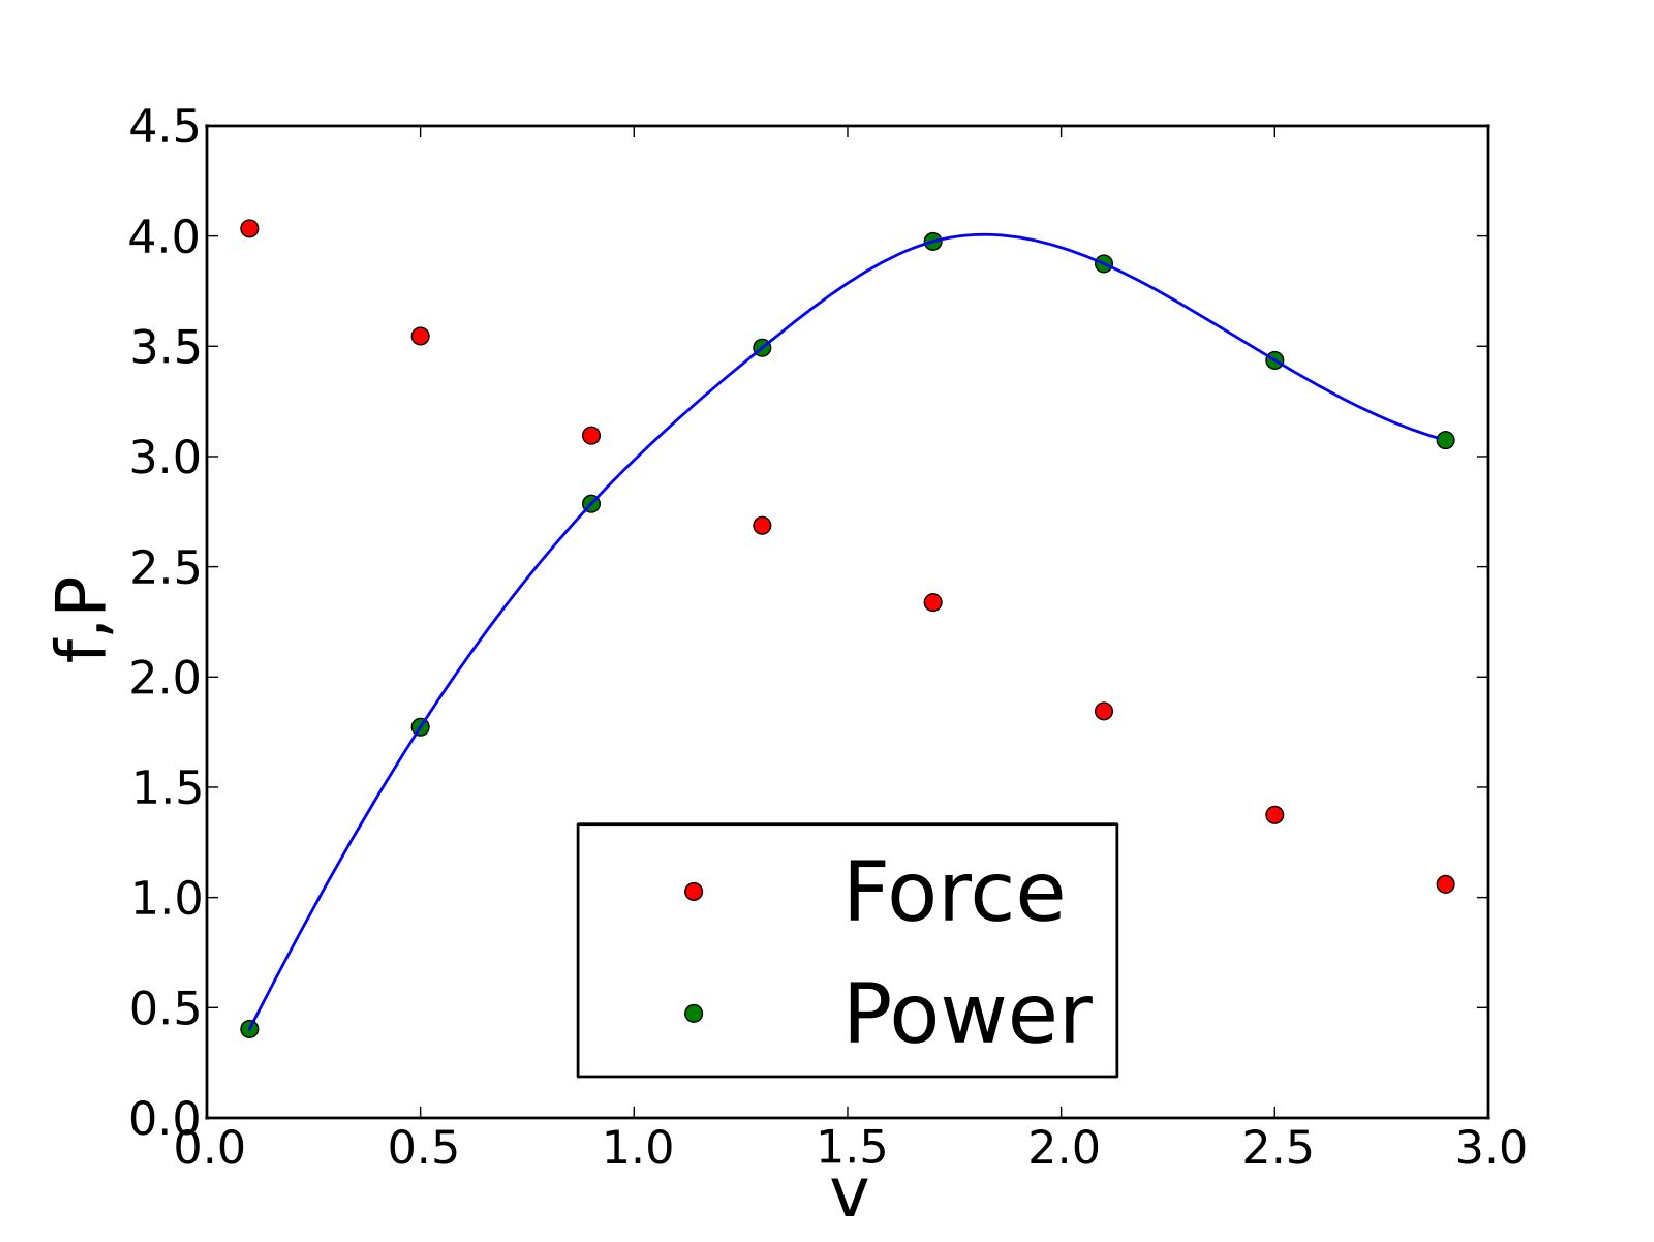
\includegraphics[width=4in]{fvsv.k15}\\
(a)\\
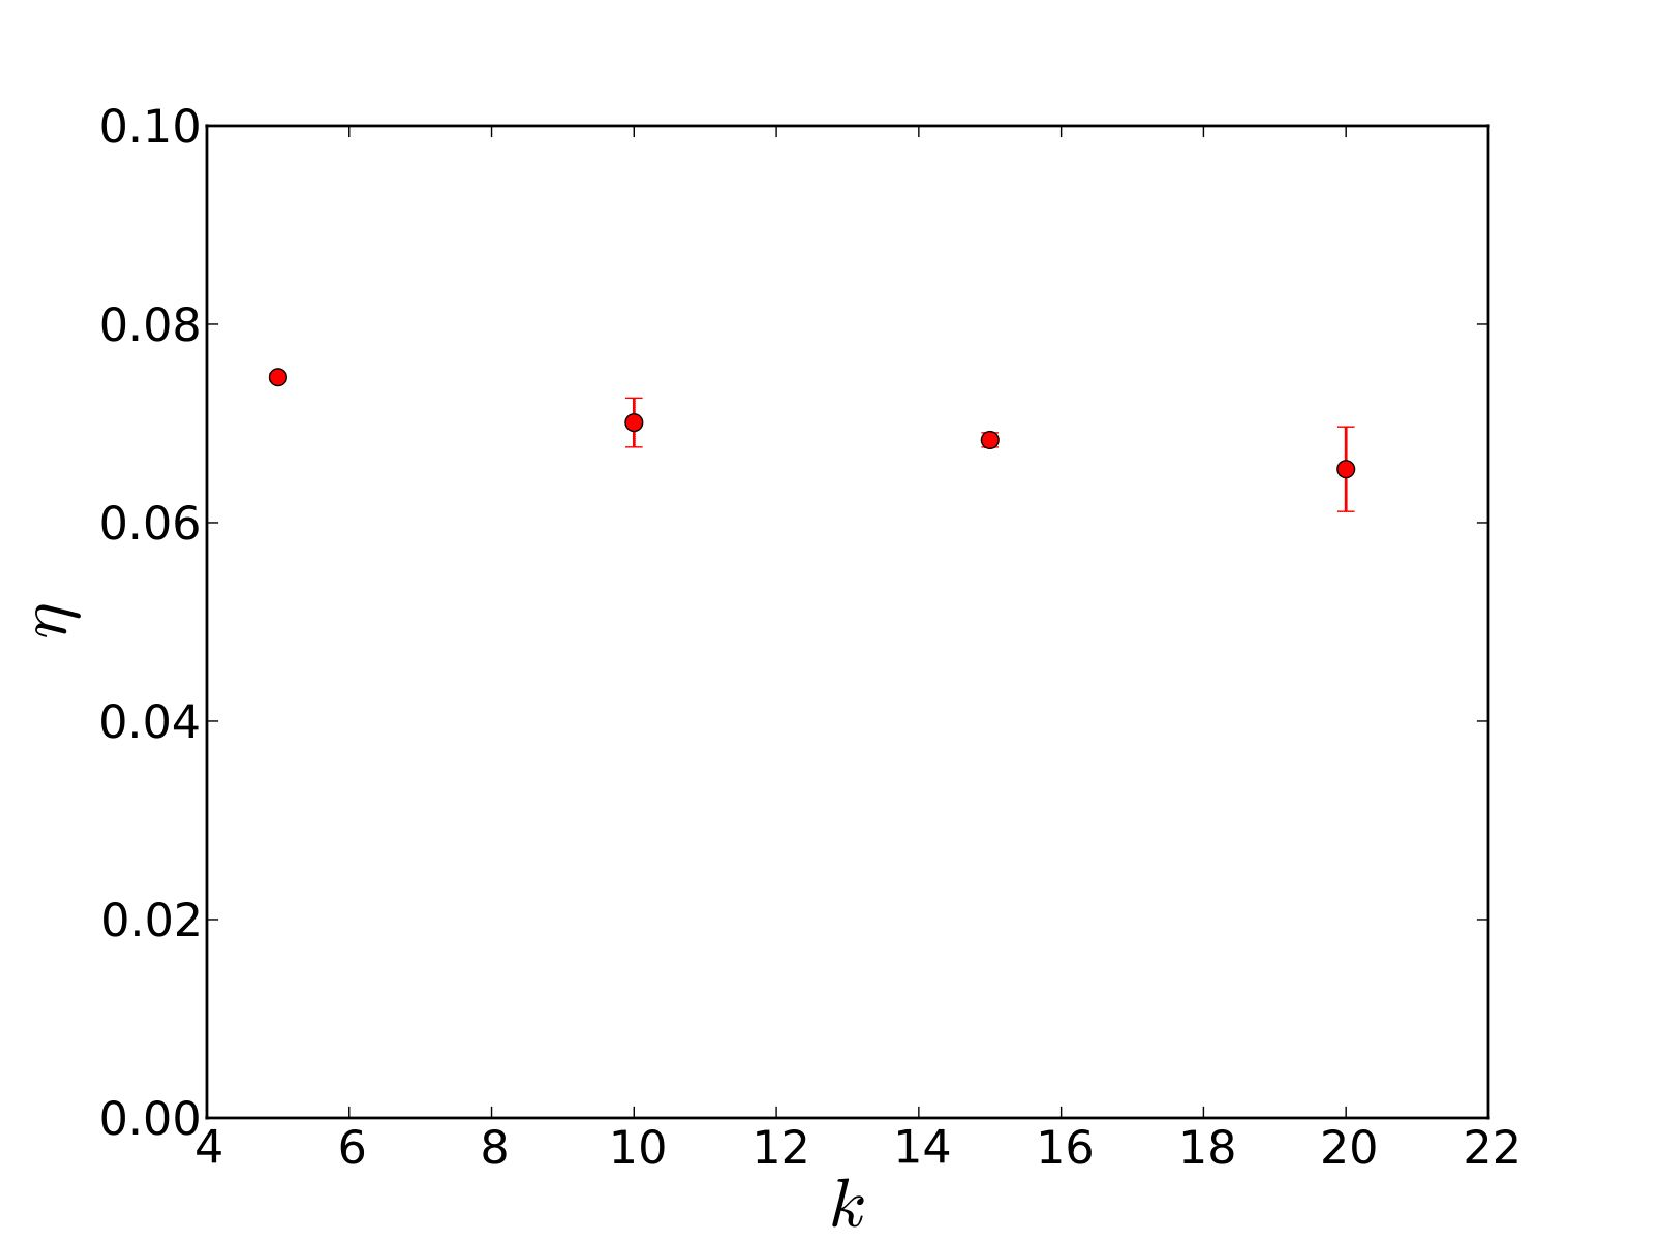
\includegraphics[width=4in]{maxpower}\\
(b)
\caption{
(a) The force and power versus velocity for the one dimensional model described
in the text. Here the spring coefficient $k=15$. The line going through the
power is a cubic spline fit used to more accurately determine the maximum value
of the power. The velocity and power are both in units of $10^{-6}$.
(b) A plot of the efficiency of the motor as a function of the spring constant
$k$. Four separate runs, each of $3\times 10^{10}$ steps were used to determine
the error bars, for each data point shown.
}
\label{fig:1dfvsv}
\end{center}
\end{figure}

We are interested in the limit of large $k$, although this is hard to achieve
numerically owing to exponentially long relaxation times. The parameters used
allow us to probe up to $k=20$. 
In the large $k$ limit, the  minimum value of $V_{min}$ needed to bind is
$k l^2 /2$, where $l$ is the maximum amount the spring will need to stretch
from the tether to the binding site. Because $\delta = 0.1$ and $L=1$, this
implies $l=0.9$. Therefore our formula for the efficiency, given this input
energy is $\eta = P_{max}/(c k l^2 /2)$, where $P_{max}$ is the maximum of the
power versus velocity, as shown in Fig. \ref{fig:1dfvsv}(a). Plotting the
efficiency for different values of $k$ ranging from $5$ to $20$ yields the
points in Fig. \ref{fig:1dfvsv}(b). 
Despite the fact that the relaxation time for metastable relaxation of the system
varies over more than two orders of magnitude, the overall efficiency is almost
constant. We expect at higher value of $k$, the efficiency will eventually drop
owing to the fact that the average unbinding time becoming smaller than the
metastable relaxation time.

What the above analysis shows is that in the limit where the photon cross section can be made arbitrarily low, the efficiency 
can be adjusted to be constant, independent of the photon energy. This is
accomplished by choosing a large spring coefficient. In reality
with photon energy of $2 eV$ and $k_B T \approx 1/40 eV$, photon flux would have
to be far too low for this optimal regime to be realizable. However the
above analysis also shows that the efficiency can be substantially increased by
choosing larger $k$ at the expense of lowering the cross section. The energy
delivered in one cycle should scale as $E_c = k L^2$. This can be increased to
be substantially larger than thermal energies but at the expense of a long
relaxation time proportional to $\exp(E_c/k_B T)$. As noted earlier, it should
be possible to make $E_c$ about $7 k_B T$, with reasonable parameter estimates. 

\section{Conclusions}
\label{sec:Conclusions}
Here we have analyzed the viability of converting photons to mechanical
energy using a device composed of an canted polymer brush tethered to a
lower plate but able to bind its other ends to sites on an upper plate. Photons can dissociate
these ends from binding sites. By a combination of analytical and numerical arguments we showed
that in steady state, this produces net mechanical power.

The system is inspired by biological motors such as myosin II that bind
to actin and dissociate via the binding of ATP. The analysis used here
could also be applied to such systems, however in reality they contain
many more stages. In general, these kind of systems are classified as 
``thermal ratchets"~\cite{ReimannRev}, where the system can be thought of as moving in a
washboard potential in the presence of thermal noise. Though that description
can be very useful in understanding the general principles behind
the operation of such motors, in the present case we are trying to model
the system in more detail than such models can afford. Instead we have described
the system using Langevin dynamics and also two coupled Fokker-Planck equations similar
in spirit but not identical to previous approaches~\cite{ProstPRL,BustamanteKellerOster}. The difference
here is that in order for potentials to be a sensible model for a polymer tethered
to a single point, they cannot be periodic. Such modelling allows us to
see how varying microscopic parameters affect the power and force
characteristics. 

The analytical results on the Unbound Equilibration Model and extensive one
dimensional simulations, show that the force
applied by the device can be made arbitrarily large at the expense of having
exponentially long relaxation times. At a given photon flux, the production of large forces 
from single polymers imply the need for a very low 
cross section of interaction between the photon and the bound end plus binding
site, as long relaxation times are required. Therefore there is a trade off between this force
and the speed the device can move. This may be circumvented to some extent by
stacking transparent devices of this kind, so that even though the cross-section of interaction of an
individual photon with a given layer is low, it will eventually be captured
by one layer. 

Therefore it appears that there is no theoretical obstacle to prevent
the photo-mechanical conversion of energy in this manner, however
it represents a significant experimental challenge. That being said, we have shown through simulations that the photomechanical effect of this device persists even when binding sites are placed randomly on the upper plate, which suggests that the precision required for production may indeed be afforded some flexibility.

It has been pointed out~\cite{GrzybowskiReview} that there is an important
distinction between artificial molecular switches and artificial molecular
machines, the former being a fraction of a penny, and the latter being extremely
challenging to create. The approach investigated here is closer to biological
motors than other proposals, and should be more forgiving about randomness, either 
in fabrication or due to thermal motion, than approaches that require precise chemical synthesis
of molecules capable of sophisticated conformational changes~\cite{credi2006}.
However, its experimental realization is still quite clearly a formidable task.

\chapter{Emergence of Metachronal Waves in Active Microtubule Arrays}

\section{Introduction}
Metachronal waves refer to the synchronization of thin, flexible
appendages that result in large-scale wavelike formations. These
appear in biological systems at the macroscopic scale (e.g. the
motion of millipede legs) and at the microscopic scale (e.g. cilia
in air pathways). On the microscopic level, metachronal waves are
essential components of several critical biological processes, from
motility in microorganisms to mucus clearance in human bronchial
tubes \cite{Afzelius2004,Okada2005}. If cilia are unable to effectively
move and synchronize, the results are often severe -- especially
if the disorder is genetic \cite{Afzelius2004}. Research into
physical explanations for cilia beating~\cite{brokaw1975molecular}, and of spontaneous metachronal behavior in cilia
is ongoing and still not well understood~\cite{camalet1999self,lindemann2010flagellar}, although many have suggested
that this phenomenon can be explained from hydrodynamic coupling
between cilia \cite{Sleigh1969,Sleigh1974,Gheber1989,Gueron1997}.

Recently, in some remarkable experiments, Sanchez et al. demonstrated metachronal wave behavior in
an \textit{in vitro} system\cite{Sanchez2011,sanchez2013engineering}.  
Microtubules (MTs) aggregated into bundles of length $10-100 \mu\mathrm{m}$ due to the addition of
polyethylene glycol~\cite{needleman2004synchrotron}.
Many of these bundles attached at one end
to a fixed boundary forming dense arrays. When exposed to a solution
containing clusters of kinesin and ATP, sustained metachronal wave
behavior between MT bundles (similar to that displayed by cilia and
flagella) was observed. MT bundles were constrained to move between
two glass slides. It is surprising that a system with such few ingredients
could develop complex behavior that so closely
resembles biological systems, which are made up from a much
more complicated machinery. Proteomic analysis indicate that eukaryotic cilia are
composed of many hundreds of proteins~\cite{pazour2005proteomic}.

Some important details of this
\textit{in vitro} system are still unclear, most notably whether the
MTs in this experiment are unipolar or of mixed polarity. 
Opposite polarity MTs will move past each other, causing separation
into unipolar bundles~\cite{kruse2000actively,liverpool2003instabilities}. 
We present arguments and simulations for unipolarity in 
\ref{app:unipolar}.
The surprising mechanism for the motion of unipolar bundles mentioned here
has not previously been given~\cite{Sanchez2011,sanchez2013engineering}, 
and we believe that the agreement between our model and
experiments provides further evidence to support our proposed explanation. 

In this article, we first outline a mechanism by which the metachronal
wave formation observed by Sanchez et al. can be understood. 
%(Section \ref{sec:mech}). 
The mechanism described here is in most ways
identical to the model used to describe and simulate cytoplasmic
streaming in \textit{Drosophila} oocytes, and the fact that it can
be adapted as such is in many ways a testament to its predictive
power. A fair amount of attention has been paid in recent years to
the understanding of how metachronal waves form in such arrays
\cite{Lagomarsino2003,guirao2007spontaneous,Elgeti2013,Niedermayer2008}. However, such
models often rely on assumptions about individual MT (or cilia)
beat patterns and/or on phenomenology. The model we propose makes
no such assumptions (beyond some minor simplifications), relying
on first-principles fluid mechanics calculations. This is important,
as it is not clear why one would additional want to impose oscillatory behavior
on individual MTs given the lack of a well defined internal structure.

%In Section \ref{sec:results}, we present the results of hydrodynamic coupling simulations which replicate the behavior observed by Sanchez et al. We also present the results of simulations with varying parameters in two different geometries. Section \ref{sec:disc} discusses the behaviors observed and compares these results to the observations of Sanchez.


%------------------------------------------------
\section{Proposed Mechanism of Action}
\label{sec:mech}


\begin{figure}
\begin{center}
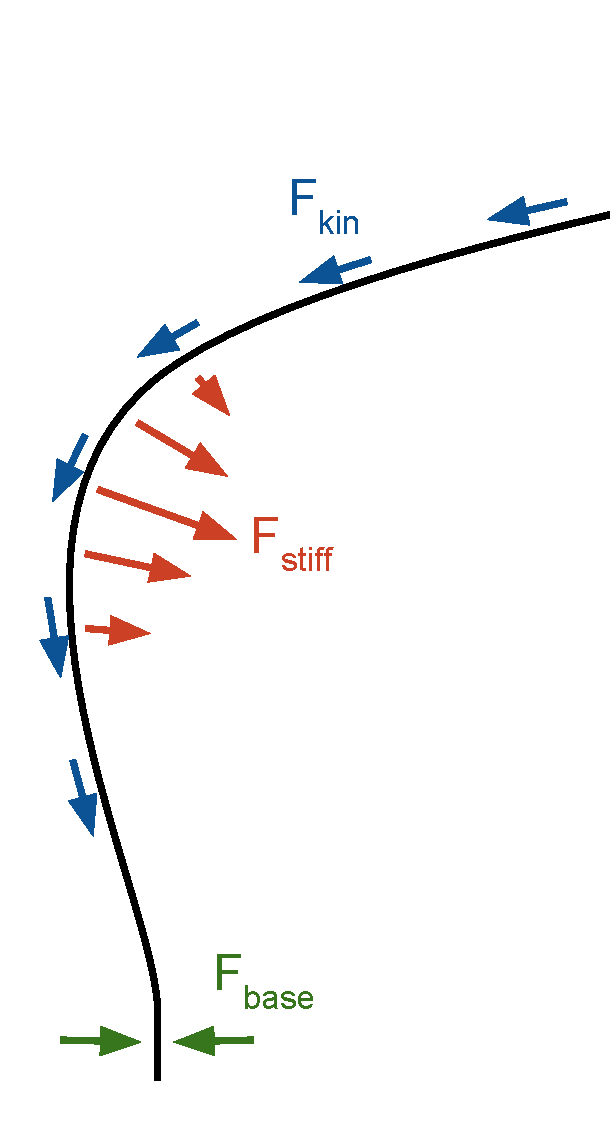
\includegraphics[width = 2in]{MT_forces}
%\captionsetup{justification=justified}
\caption{Conceptual illustration of forces acting on a single polymer
that are not due to hydrodynamic interactions. The blue vectors
indicate the buckling forces due to kinesin walkers (tangent to
polymer), the red vectors show the direction and relative magnitude
of stiffness forces (in the direction of $d^4\mathbf{r}/ds^4$), and
the green arrows indicate a restorative force keeping the base of
the polymer approximately perpendicular to the binding
surface.
\label{fig:Mtforces}
}
\end{center}
\end{figure}


We now present a model for the simulation of the Sanchez
et al. system. A similar method has been used successfully to
simulate cytoplasmic streaming in \textit{Drosophila}
oocytes\cite{Monteith2016}, and is based on theoretical
work completed several decades ago regarding the calculation of
Stokes flows created by a point force (stokeslet) near no-slip
boundaries\cite{Blake1971,Liron1976}. A conceptual explanation of
this mechanism is given below, and further details regarding theory
and implementation are given in \ref{app:2Dint} and
\ref{app:sim}.

An illustration of how MT bundles are simulated is given in Figure
\ref{fig:Mtforces}. Each MT bundle is modeled as a chain of monomers
(i.e. polymer) which are held an approximately fixed distance from
one another by a spring force. The base of each polymer is anchored
to a single point, and the polymer at the base is kept roughly
perpendicular to the anchoring surface. Let the polymer be described
by the curve $\mathbf{r}(s)$, where $\mathbf{r}(0)$ is the location
of the polymer base, and $s$ is the arc length. We give the polymer a stiffness by implementing
an energetic cost of bending proportional to curvature squared, which
implies a local force at $s$ proportional to  $d^4\mathbf{r}/ds^4$. Additionally, monomers feel a ``buckling"
force due to the drag from the walking kinesin $F_{kin} = - f_k d\mathbf{r}/ds$, which is parallel to the polymer
and toward the polymer base. $f_k$ will depend linearly on the speed of the kinesin
and the solvent viscosity. This force continually adds energy to
the system (making it active), and has been shown to be a good
representation of the average drag force due to kinesin walking
along the microtubule away from the polymer base~\cite{Monteith2016}.

This kind of model for a single chain was first employed to understand glide assay dynamics
in two dimensions~\cite{bourdieu1995spiral}. In three dimensions,
periodic waves develop whose dynamics have been analyzed in detail~\cite{Monteith2016}, and
related theoretical work has recently also been performed~\cite{de2017spontaneous}. However,
scaling can be used to get the relevant length and timescales~\cite{bourdieu1995spiral}.
The average radius of curvature depends on the strength of the buckling force $f_k$,
and the elastic constant of a filament characterizing its stiffness $k_{stiff}$. The radius of curvature over
quite a wide range of parameters can be shown to be
$R = (k_{stiff}/(\beta f_k))^{1/3}$, where $\beta \approx 0.05$. Likewise, the angular frequency is
$\omega = f_k/(\nu R)$, where $\nu$ is the hydrodynamic drag coefficient per unit length.
Although there is a fairly large experimental uncertainty in parameters
used to model a Drosophila oocyte, this model finds quite good agreement with the experimental
time and length scales. $R$ was predicted to be $25-54\mu$m, close to the $16.3\pm 2.2 \mu$m observed.
Likewise, the time scale was predicted to be $203-1094$s, which is in the observed range of $370\pm 42$s.
It is interesting that the length and time scales observed by Sanchez et al. are also quite close to
these numbers, and that the frequency of biological cilia beating is often three orders of magnitude higher than this.


Polymers also feel hydrodynamic forces.
As the force from the kinesin causes the polymers to buckle, we
begin to see complex motion. Each monomer acts as a point force
(stokeslet) in the surrounding fluid. This force a monomer exerts
on the fluid is simply the sum of all of the other forces on the
monomer: because the Reynolds number is nearly zero, there are no
inertial terms, meaning the force is transferred perfectly from the
monomer to the fluid. As this is a Stokes flow, the flow contributions
from all stokeslets add linearly, and we can (in principle) calculate
the flow everywhere. However, we do not need to calculate the fluid
velocity everywhere -- only at points with monomers. 
%As such, the
%results of what initially seems to be a computationally intense
%fluid mechanics calculation 
Therefore, the evolution can be calculated via a pairwise sum over
all monomers (see \ref{app:2Dint}).

We also assume all polymer motion is two dimensional with a constant value of $z$, which
is physically sensible when considering the geometry of the Sanchez et al.
experiments. In this experiment, MT bundles were observed between
glass slides, with a height $H$, of approximately $10 \mu$m, creating a narrow channel for which fluid can flow.
For this reason, we adopt a two dimensional geometry. In addition,
the no-slip boundaries
of the plates have a large impact on the hydrodynamic forces between
monomers\cite{Blake1971,Liron1976}, which we state explicitly in \ref{app:2Dint}. Other close-range contact forces were
also used (repulsion from anchoring surface, monomer-monomer
repulsion), and these are explained in \ref{app:sim}.

We can now address at the qualitative level the mechanism by which
we propose the metachronal waves observed by Sanchez et al. form.
As kinesin walk away from the polymer bases, the polymers will tend
to buckle. If a polymer is isolated, this buckling will lead to
unstable motion (corkscrew motion or irregular
beating)\cite{Monteith2016}. When placed in an array,
however, nearby polymers will exert hydrodynamic forces on one
another that tend to synchronize their motion. If these hydrodynamic
forces are sufficiently strong, this can cause a transition from
disordered motion to aligned MTs and correlated motion. 

Despite the fact that this model was developed to explain and
simulate cytoplasmic streaming, its mechanism 
can be easily adapted for related biological phenomena. Indeed,
when the conditions of the Sanchez et al. experiment are simulated
in the same way, we observe metachronal waves.
It is not clear if this is formally a transition or a more continuous
crossover effect, but the results found make strong predictions
that should be testable experimentally.
In the following, we present
the results of these simulations and discuss the required conditions
for metachronal wave formation. 


%------------------------------------------------

\section{The Quasi-2D Interaction Tensor}
\label{app:2Dint}
\begin{figure*}
\begin{center}
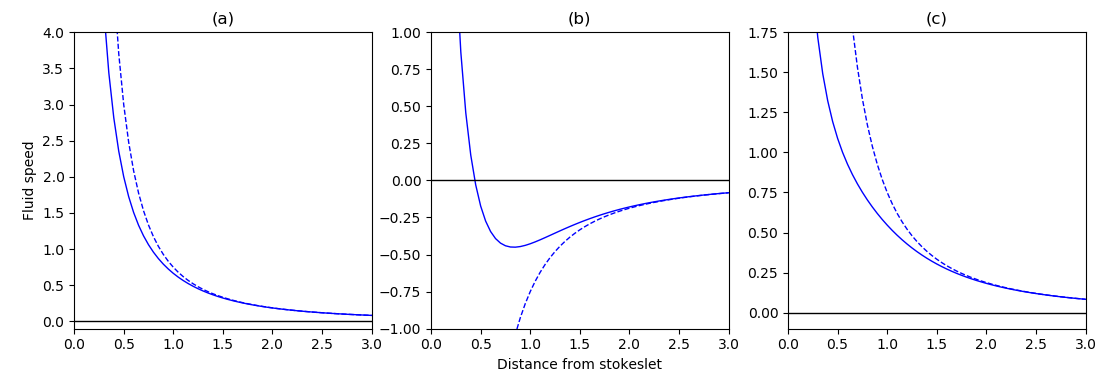
\includegraphics[width=\textwidth]{Sec2}
\caption{Fluid speeds as a function of distance $\rho$ from the stokeslet $\mathbf{F} = \hat \imath$. Solid curves are calculated using the full interaction tensor (\ref{eq:uab}) and dashed lines are the far-field approximation (\ref{eq:uff}). (a) $u_x(\rho)$ along the line $y=0$; (b) $u_x(\rho)$ along the line $x=0$; (c) $u_y(\rho)$ along the line $y=x$. \label{fig:oseen}}
\end{center}
\end{figure*}
The interaction tensor used in simulations is that of a stokeslet enclosed by two infinite parallel plates, as derived by Liron and Mochon\cite{Liron1976}. In general, the interaction tensor $\mathbb{G}$ is defined as the relationship between the fluid flow $\mathbf{u(r)}$ and the stokeslet $\mathbf{F}$ which causes this flow:
\begin{equation}
\label{eq:oseen}
\mathbf{u(r)} = \mathbf{F}\cdot\mathbb{G}(\mathbf{r})
\end{equation}
For computational efficiency, we assume all monomers to be only in
the $xy$-plane, with parallel plates at $z = \pm H/2$. This reduces
a three-dimensional problem to two dimensions, as (a) the stokeslet
is located in the $xy$-plane, (b) the stokeslet's direction has no
$z$-component, and (c) we only concern ourselves with flows in the
$xy$-plane (see Figure \ref{fig:schem}). For
this arrangement, it can be shown from Liron and Mochon's general
result that the interaction tensor a displacement $\mathbf{r}$ (and
$\rho\equiv|\mathbf{r}|$) from a single stokeslet $\mathbf{F}$ at
the origin reduces to
\begin{equation}
\label{eq:uab}
\mathbb{G}(\mathbf{r}) = \frac{H}{8\pi\mu\rho^2}\left\{\left[4\left(\frac\rho H\right)^2 S_1 - \frac12\frac\rho H I_1\right]\mathbb{I}+\left[4\pi\left(\frac{\rho}{H}\right)^3 S_2 + \frac{1}{2}\frac\rho H I_1 -\frac14\left(\frac\rho H\right)^2 I_2\right]\frac{\mathbf{r\otimes r}}{\rho^2}\right\}
\end{equation}
where
\begin{align*}
S_1\equiv&\frac14\sum_{n=0}^\infty \frac{(-1)^n}{\left[\left(\frac{\rho}{H}\right)^2 + n^2\right]^{1/2}}\\
S_2\equiv&\frac{1}{4\pi}\frac\rho H\sum_{n=0}^\infty \frac{(-1)^n}{\left[\left(\frac{\rho}{H}\right)^2 + n^2\right]^{3/2}}\\
I_1\equiv&\int_0^\infty \xi J_1\left(\frac\rho H \xi\right)\frac{\tanh^2\frac\xi 2}{\sinh\xi - \xi}d\xi\\
I_2\equiv&\int_0^\infty \xi^2\left[J_0\left(\frac\rho H \xi\right) -J_2\left(\frac\rho H \xi\right)\right]\frac{\tanh^2\frac\xi 2}{\sinh\xi - \xi}d\xi
\end{align*}
Here, $J_n$ is the Bessel function of the first kind. Because $S_1$ and $S_2$ do not converge rapidly as defined above, we also make use of the Poisson sums
\begin{align*}
S_1 =& \sum_{k=0}^\infty K_0\left[\pi(2k+1)\frac\rho H\right]\\
S_2 =& \sum_{k=0}^\infty (2k+1) K_1\left[\pi(2k+1)\frac\rho H\right]
\end{align*}
where $K_n$ is the modified Bessel function of the second kind.

In the far field, it can be shown that (\ref{eq:uab}) approaches
\begin{equation}
\label{eq:uff}
\mathbb{G}\mathbf{(r)} \approx -\frac{3H}{32\pi\mu\rho^2}\left(\mathbb{I} -2\frac{\mathbf{r\otimes r}}{\rho^2}\right)
\end{equation}
Figure \ref{fig:oseen} shows plots of $\mathbf{u(r)}$ at selected locations, and compares the exact value from (\ref{eq:uab}) to the far-field approximation from (\ref{eq:uff}).

We can now make some conceptual observations regarding this interaction tensor and how it compares to the boundary-free Oseen tensor $\mathbb{G}_0$:
\[
\mathbb{G}_{0}(\mathbf{r}) = \frac{1}{8\pi\mu r}\left(\mathbb{I} + \frac{\mathbf{r\otimes r}}{r^2}\right)
\]
First, we immediately notice a $1/r$ dependence (rather than $1/\rho^2$). This means forces without boundaries tend to be more long-range, and boundaries result in long-range screening. Second, $\mathbb{G}_{0}$ is always positive, whereas this is not true for the interaction tensor used here. One key implication of this is that flows created by a stokeslet are often flowing opposite its direction (e.g. Figure \ref{fig:oseen}b). Both of these qualities may enhance metachronal behavior in the confined system. Screening means that interactions between nearby polymers are most important, creating a ``domino effect" from one polymer to the next rather than having motion more influenced by long-range interactions. The creation of opposing flows means (among other things) that if one polymer is moving toward the anchoring surface, it may exert a force on many of its neighboring polymers \textit{away} from the anchoring surface. This encourages wavelike behavior rather than uniformity of beating motion.


\begin{figure}
\begin{center}
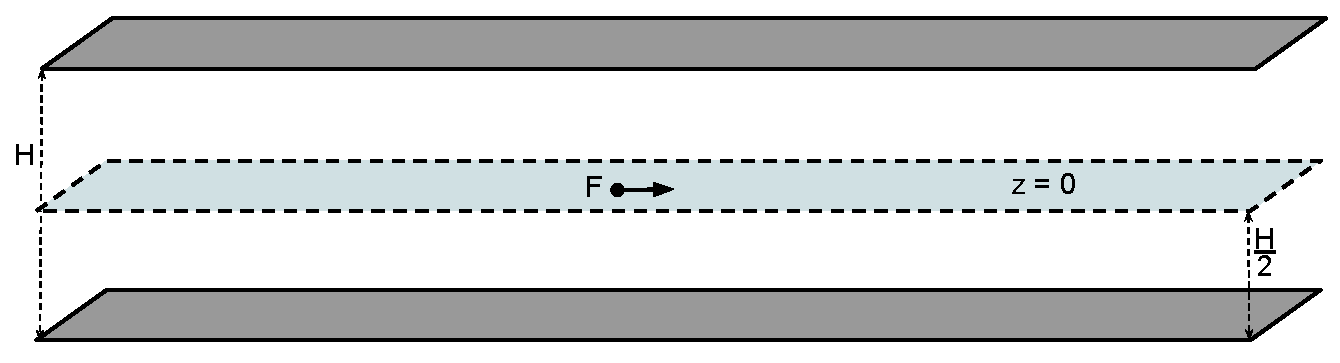
\includegraphics[width = \textwidth]{2plates}
\caption{Illustration of the geometry for which interaction tensor
is derived in \ref{app:2Dint}. While this is a three-dimensional
system, we constrain polymers to the $xy$-plane. 
\label{fig:schem}}
\end{center}
\end{figure}

\section{Simulation Methods}
\label{app:sim}

\begin{figure}
\begin{center}
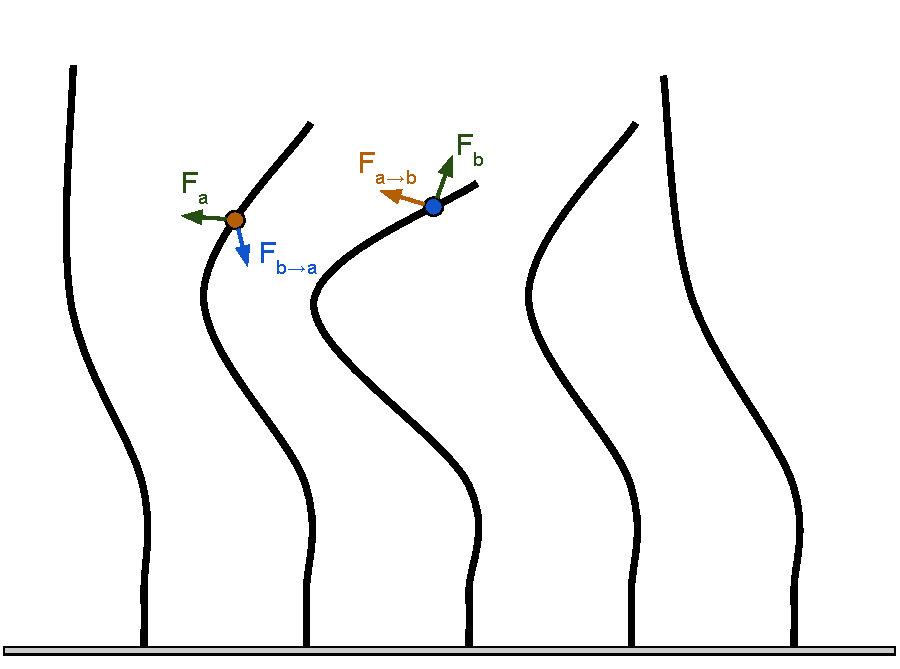
\includegraphics[width = 4in]{hydroforces}
\caption{Illustration of hydrodynamic forces between two example
monomers in a planar polymer array. The green forces are the sum
of non-hydrodynamic forces on the monomer (and by extension the
force the monomer exerts on the surrounding fluid). $\vec F_{a\rightarrow
b}$ and $\vec F_{b\rightarrow a}$ are the hydrodynamic forces on
monomer $b$ due to $\vec F_a$ and the hydrodynamic force on monomer
$a$ due to $\vec F_b$, respectively. 
\label{fig:hydroforces}}
\end{center}
\end{figure}

The algorithm we implement is built on work that was used to
simulate the mechanism behind cytoplasmic streaming in \textit{Drosophila}
oocytes \cite{Monteith2016}, and many of the methods and equations
below are explained in detail in these papers. This software simulates
an array of active microtubules tethered to a plane that works as follows
and is explained in further detail below.
\begin{enumerate}
\item After an array of polymers is initialized, forces on all
monomers are summed (described below, also see Figure
\ref{fig:Mtforces}) and monomer position and
velocity are updated using time step $dt$.
\item This motion initiates complex flow in the surrounding fluid.
The fluid flow is not simulated directly, but the resulting
hydrodynamic forces from this flow are calculated via an Oseen
tensor with corrections by Blake\cite{Blake1971}. This is illustrated in Fig. \ref{fig:hydroforces}.
\item Forces on each monomer are summed, and monomer position and
velocity are updated accordingly.
\item Once updated, steps 2-3 are repeated.
\end{enumerate}
In the present work there were these differences: 
\begin{enumerate}
\item $N$ Microtubules are confined to the $xy$-plane, with polymer
bases separated by a distance $l$ tethered either to a flat plate
at $y=0$ or to a circular boundary. For all presented results,
$N=128$. The geometry of this is shown in Fig. \ref{fig:schem}.
\item At the tethering point, a potential was added in order to
keep the base monomer approximately orthogonal to the boundary.
\item Rather than the Blake correction to the Oseen tensor, we use
the simplified Liron/Mochon interaction tensor described in Section
\ref{app:2Dint}.
\end{enumerate}

\noindent
Now we describe how the above was accomplished in more detail.
Each polymer is composed of $n=16$ monomers. The $i$th monomer
position $\mathbf{r}_i$ is updated a using a fourth order Runge
Kutte integration of the equation
\begin{equation}
\frac{d\mathbf{r}_i}{dt} = \mathbf{u(r}_i) - k_{kin}\left(\textbf{r}_{i-1} - \textbf{r}_{i+1}\right)
\end{equation}
where $dt$ is the time step (set to 0.003), $k_{kin}$ (set to 0.2)
controls the strength of the kinesin force tangent to the polymer
($\mathbf{F}_{kin}$ in Figure \ref{fig:Mtforces}), and $\mathbf{u(r}_i)$
is the fluid velocity due to the motion of all other monomers as
given by Equation \ref{eq:oseen} and \ref{eq:uab} (which imparts
the forces $\mathbf{F}_{a\rightarrow b}$ in Figure \ref{fig:hydroforces}):
\begin{equation}
\mathbf{u(r}_i) = \sum_{j\neq i} \mathbf{F}_j \cdot \mathbb{G}(\mathbf{r}_i-\mathbf{r}_j)
\end{equation}
Here, $\mathbf{F}_j$ is the total force on the fluid due to the $j$th monomer. Because there are are no inertial effects when $Re\ll 1$, any non-hydrodynamic force exerted on the monomer must be transferred to the fluid. In our case,
\begin{equation}
\mathbf{F}_j = \mathbf{T}_j + \mathbf{C}_j + \mathbf{Q}_j,
\end{equation} 
where
\begin{itemize}
\item $\mathbf{T}_j = k_{spr}\left[\left(|\mathbf{r}_{j-}|-\ell\right)\hat{\mathbf{r}}_{j-} + \left(|\mathbf{r}_{j+}|-\ell\right)\hat{\mathbf{r}}_{j+} \right]$\\
with $\mathbf{r}_{j\pm}\equiv \mathbf{r}_{j\pm 1} - \mathbf{r}_j$, is the spring force keeping monomer separation approximately constant. For our simulations, $k_{spr}=100$ and $\ell=1$.
In these simulations the separation between polymer bases defines above, $l$ is equal to $4\ell$.
\item $\mathbf{C}_j = k_{stiff}\left(2\textbf{r}_i - \textbf{r}_{i+2} - \textbf{r}_{i-2}\right)$\\
is the stiffness force which resists polymer bending. $k_{stiff}$ is varied in our simulations, but typically $5 \leq k_{stiff} \leq 20$.
\item $\mathbf{Q}_j = \mathbf{P}_j + \mathbf{B}_j + \mathbf{W}_j + \sum_k\mathbf{H}_{jk}$\\
is the sum of miscellaneous conditional forces:
\begin{itemize}
\item $\mathbf{P}_j = k_{pin}\left(\mathbf{r}_j - h\boldsymbol{\hat{\jmath}}\right)$\\
\phantom{.}\hfill if $(j \mod n) = 1$\\
is the force on the base monomer of each polymer chain keeping it pinned to the anchoring surface. For our simulations, we set $k_{pin} = 100$ and $h=1$.
\item $\mathbf{B}_j = k_{pin2}\left(\mathbf{r}_j - \mathbf{r}_{j-1} - \ell\boldsymbol{\hat{\jmath}}\right)$\\
\phantom{.}\hfill if $(j \mod n) = 2$\\
is the force on the second monomer in each polymer chain, keeping
the base of each polymer approximately orthogonal to the anchoring
surface ($F_{base}$ in Figure \ref{fig:Mtforces}). For our simulations,
we set $k_{base}=100$.
\item $\mathbf{W}_{j} = k_{wall}\left[1-\left(\frac{d_{wall}}{y_j}\right)^4\right]\boldsymbol{\hat\jmath}$\\
\phantom{.}\hfill if $y_j < d_{wall}$\\
is the repulsive force exerted by the anchoring plane on any monomer that gets close to the wall. For our simulations, we set $d_{wall}=0.5$ and $k_{wall} = 100$.
\item $\mathbf{H}_{jk} = k_{rep}\left[1-\left(\frac{d_{rep}}{|\mathbf{r}_j - \mathbf{r}_k|}\right)^4\right]\left(\mathbf{r}_j - \mathbf{r}_k\right)$\\
\phantom{.}\hfill if $|\mathbf{r}_j-\mathbf{r}_k| < d_{rep}$\\
is the repulsive force between monomers that are very close to one another. For our simulations, we set $d_{rep}=0.5$ and $k_{rep} = 1$.
\end{itemize}
\end{itemize}
\section{Analysis of Unipolarity}
\label{app:unipolar}

The work of Sanchez et al.~\cite{Sanchez2011,sanchez2013engineering} consists of a mixture of 
biotin-labeled kinesin-1 motors bound together to form clusters using multimeric streptavidin
and taxol stabilized microtubules in a polyethylene-glycol solution with
ATP. These form bundles of microtubules, some of which are adsorbed to
air-water or air-glass interfaces, that point out from the interface forming a
lawn of microtubule bundles. These bundles are flexible and show bending similar
to what is seen in the simulations described here
in both the time scales, length scales, and correlations
between different bundles.

The question that is not answered in the experimental work is the directionality
of the microtubules inside a bundle. The microtubules forced into bundles by the polyethylene glycol (PEG)
could be of mixed polarity
so that some have their minus ends at the interface while others have their plus
ends there. We will refer to microtubules with different orientations as having
different ``polarities", minus-ends against the interface as ``minus" and those with opposite
polarity as ``plus". 

The problems with having a mixed polarity bundle are two fold. The first is
that for a wide range of experimental parameters, we expect mixed polarity 
bundles to be unstable~\cite{kruse2000actively,liverpool2003instabilities}. The second problem is that it is not clear that
mixed polarity bundles can give rise to the motion seen experimentally. We
will analyze both problems below.

\subsection{Instability of mixed polarity bundles}

The first problem is that adjacent
microtubules with different polarities will be linked by kinesin clusters that
will apply equal and opposite forces to them. This will cause the minus
microtubules to be pushed toward the interface, and the plus ones away from it. 
The forces from the kinesin act in parallel on a microtubule over its length
which is of order $10 \mu m$.
The forces that these cause can be competitive with depletion forces caused by the
PEG as we will now see.
A full analysis of this is not possible without more information
about the details of the system such as the density of kinesin clusters and chain
lengths of the PEG. However we can do a calculation to show that even with
very modest assumptions concerning kinesin density, expulsion of plus
microtubules will take place.

Depletion forces exert an osmotic pressure on microtubules and filaments. 
Each polymer excludes a roughly spherical region of order its radius of
gyration $R_g$.
Entropic forces favor the separation of microtubules into bundles because less
volume is excluded by the PEG. We will estimate the force acting on a
single microtubule protruding from a bundle. 
PEG is depleted in a region of size $R_g$ around the microtubule. The increase in
free energy per unit area caused by this depletion is of order $p R_g$  where the osmotic pressure is  $p = k_B T \rho$, and
$\rho$ is the number of polymers per unit volume. The increase in free energy
$dF$, in raising the microtubule by a height $dz$, is $dF = (2\pi R_m dz) p x$. Here $R_m$
is the microtubule radius. If we assume that the
polymers are close-packed around the microtubule to get the maximum effect, then $\rho = 1/(4 \pi R_g^3/3)$.
So the force needed to push the microtubule out of the tip of the bundle is
$f = dF/dz = (3/2) R_m k_B T/R_g^2$.

$R_m \approx 13 nm$ and conservatively taking $R_g = 1nm$, which is quite small
for PEG, $f = 81 pN$
The stall force of kinesin is approximately $5pN$~\cite{meyhofer1995force}. So only 16.2 kinesins are needed to overcome
the depletion forces and expel this microtubule from the bundle. 

The minimum separation of kinesin on a microtubule is $8nm$ and there are 13
tracks around its circumference. Because kinesin has a strong affinity for
microtubules we expect a high density of bound kinesin. Therefore 16 kinesins
contributing to the force over
a distance of $10 \mu m$ is over three orders of magnitude less dense
than the maximum density attainable.
This suggests that for a wide range of parameters, the microtubule bundles will
become unipolar with minus-ends against the interface.


\subsection{Model of mixed polarity bundles}

The second problem is
that it is not clear that a mixed polarity bundle can give rise to the motion
seen in experiment. Here we analyze this possibility by using simulation methods
similar to what was used previously to understand molecular motor dynamics~\cite{deutsch2015photomechanical}

We assume that the microtubules are inextensible and that opposite polarity
microtubules apply forces in equal and opposite directions. We discuss the
different forces separately.

First there is an effective attractive interaction between microtubules independent of 
their polarities induced by the presence of PEG polymers. We choose a short range force so the monomers separated by a
distance $\br$  within a range $\sigma_s$ will feel an attractive force due to
depletion forces as discussed above. To
simplify the expressions we use a normalized unitless distance $\Delta \equiv
\br/\sigma_s$.
The force between any two monomers for $\Delta < 1$ is taken to be
\begin{equation}
{\bf f}_{attr} = f_a \Delta^4 (1-\Delta^{12})^3 \br
\end{equation}
where $f_a$ is the strength of the attractive interaction.
The reason for choosing this functional dependence on $\Delta$ was to produce
a force that was close to constant for $\Delta < 0.6$, and then drop
smoothly to zero, so as to work well with the Runge Kutte algorithm.

Second, we introduce an even shorter range repulsion between monomers
that diverges at a hard core radius $\sigma_h$ and goes to zero at $\sigma_s$:
\begin{equation}
{\bf f}_{rep} = f_r\left(\frac{1}{r^2-\sigma_h^2}- \frac{1}{\sigma_s^2-\sigma_h^2}\right)^4 \br 
\end{equation}
where $f_r$ is the strength of the repulsive interaction.

Third, we introduce an equal and opposite forces between monomers on opposite polarity microtubules
that are within a distance $\sigma_s$.
The direction of the force is as follows. We compute the tangents to both
monomers as $(\br_{i+1}-\br_{i-1})/2$. Then we choose the direction $\bf t$, to be the
average of these two tangents. The magnitude of the kinesin force is
\begin{equation}
{\bf f}_{kin} = f_k (1-\Delta^{12})^3 
\end{equation}
where $f_k$ is similar the symbol used previously and denotes the magnitude of
the kinesin force.

These forces are added to the elastic forces, viscous drag, and tension that
must be introduced to conserve link length and the equation of motion is iterated
using a method for updating chains with constant link length~\cite{deutsch1988theoretical,deutsch1989theoretical}.

We also tried two separate kinds of boundary conditions. First, tethering the chains to
fixed points on the surface which we will call ``fixed" boundary conditions. Second, confining the chain ends to a two
dimensional plane but letting the ends move within that plane, which we will
call ``sliding" boundary conditions. 

We tried a wide range of parameters, of different elastic constants, attractive
interactions, number of microtubules, and boundary conditions. What we found is
now summarized. 

For two chain bundles of opposite polarity we did find a set of parameters which
showed movement of the bundle with: 
$f_r =  10.0$, $\sigma_s =  2$, $\sigma_h = 1$, $f_a =  3$, $f_k = 0.2$, $C=
100$, and chain length of $20$.

For larger bundle sizes, e.g. 9 chains,  we did not find anything similar to
experiments. With fixed boundary conditions, and started as a pillar of
parallel microtubules with slightly randomized directions, the chains would settle down to
a pillar shape that would not change with time for sufficiently small attractive
interactions $f_a$, but when this became greater than a certain value that
depends on elastic constant and other parameters, it would suddenly collapse
into a ball because this is more highly favored energetically.

When we chose sliding boundary conditions, and for sufficiently weak attractive
interactions, $f_a=1$ there was a regime where there was twisting motion inside the
pillar but then the minus microtubules would suddenly slide off of the plus
ones, finally lying close to parallel with the plane of attachment, see supplemental movie S10. 
It therefore appears that a two microtubule bundle moves because of a strong
anisotropy in forces seen in cross sections. In larger bundles, the forces
through the bundle are more homogeneous which acts to stabilize them.

We conclude that by direct physical modeling of a mixed polarity bundle, it is
not clear if there are any reasonable parameters which show motion similar to
what is seen in the experiments of Sanchez et al~\cite{Sanchez2011,sanchez2013engineering}.

Note that the elastic constant of a microtubule in a bundle will depend strongly on the
rate at which it is bent. For very short times, the bonds between different
microtubules caused by kinesin binding will be fixed in position giving the bundle the
elastic constant of a cylinder of radius $R$ which is $\propto R^4$. However the
oscillations here take place on minute timescales. In that case the individual
kinesin molecules have velocities of order $1\mu m/s$ so 
they unbind and move very far
on this time scale. This allows neighboring microtubules to move relative to
each other, to eliminate stress. Therefore on sufficiently long timescales,
this reduces the elastic constant of a microtubule to that of one in isolation.


\section{Results}
\label{sec:results}

\begin{figure}
\centering
\subfloat[][]{
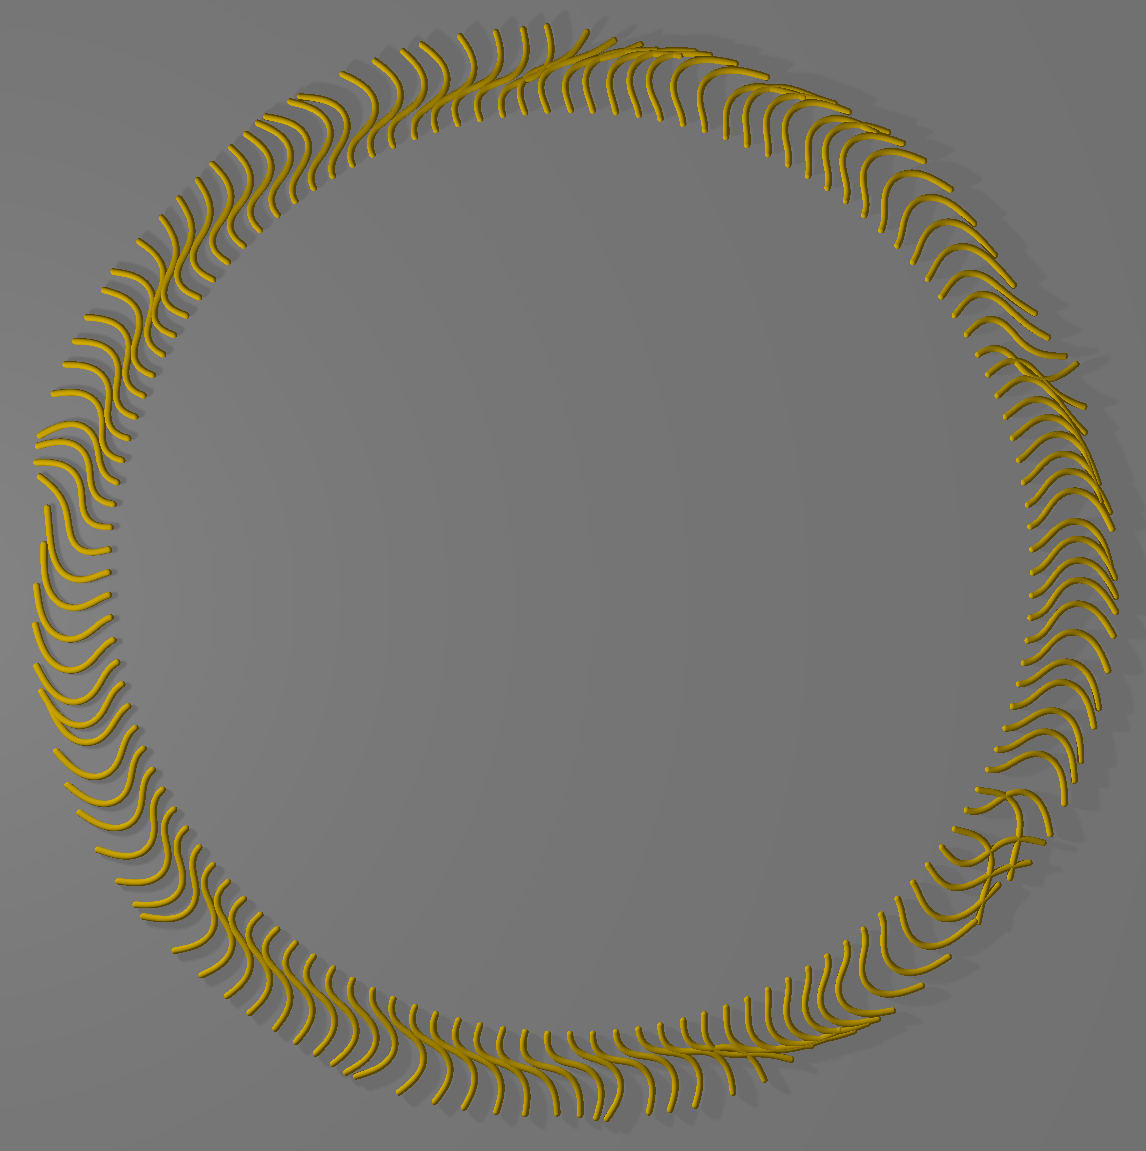
\includegraphics[width =\columnwidth]{anim_circ}
}
\qquad
\subfloat[][]{
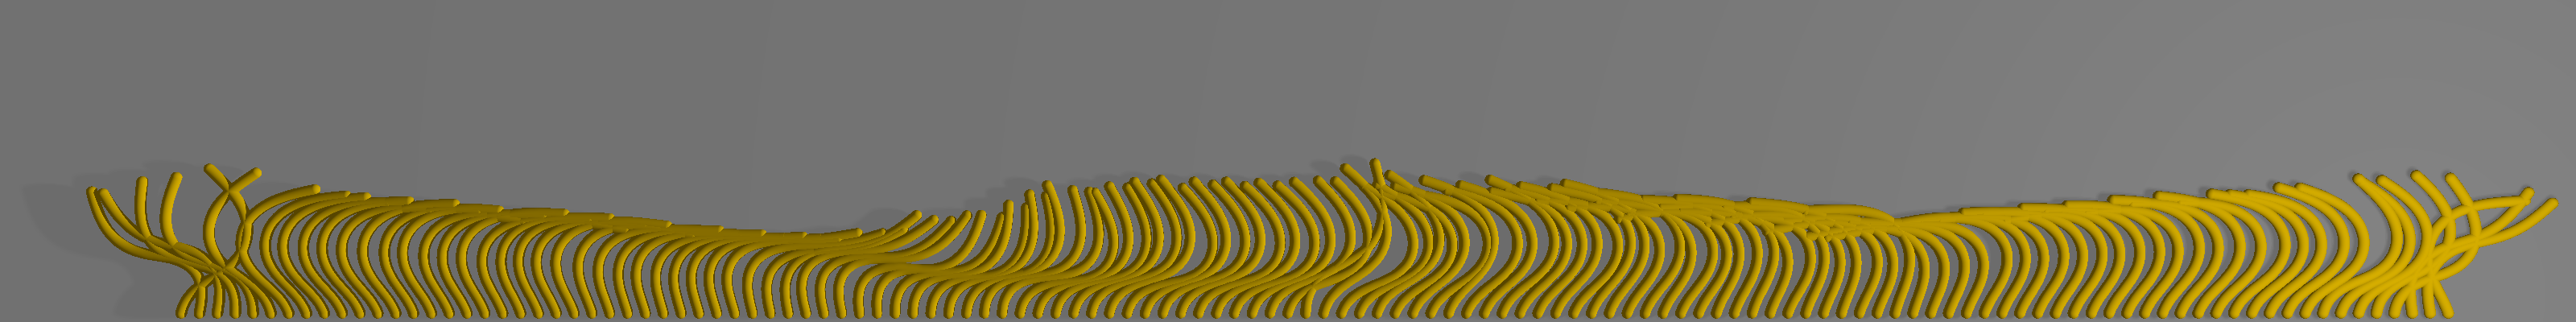
\includegraphics[width =\columnwidth]{anim_plane}
}
\caption{Simulated metachronal wave formation for 128-polymer arrays in (a) circular and (b) planar geometries. 
In both cases, $k_{oseen} = 0.1$, $k_{stiff}  = 10.0$, $H=1$.
\label{fig:anims}}
\end{figure}
Videos of select simulations are included in the Supplementary
Materials. Figure \ref{fig:anims} shows some still frames of simulated
arrays demonstrating metachronal wave behavior in both the planar
and circular geometries.

%\begin{figure}
%\centering
%\begin{subfigure}[b]{0.45\columnwidth}
%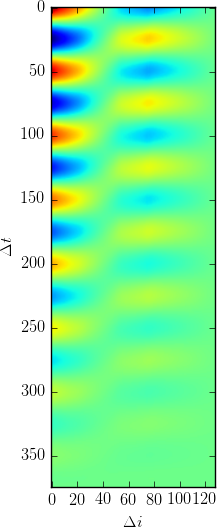
\includegraphics[height = 3in]{plane-0p1-10-4.png}
%\caption{}
%\end{subfigure}
%\begin{subfigure}[b]{0.45\columnwidth}
%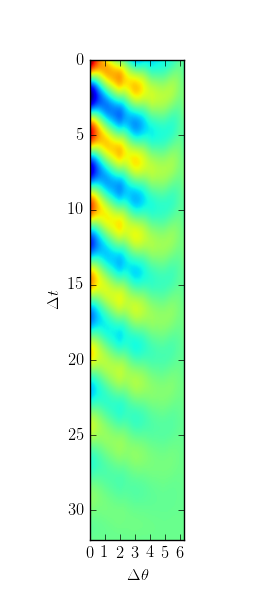
\includegraphics[height = 3in]{circ-0p2-10-4.png}
%\caption{}
%\end{subfigure}
%\caption{Characteristic correlation functions demonstrating wavelike behavior in (a) planar and (b) circular geometries. 
%\label{fig:corr1}}
%\end{figure}

We characterize the behavior of each system using the correlation function 
\begin{equation}
C(\Delta i, \Delta t) = \langle \Delta x(i + \Delta i, t+\Delta t)\Delta x(i,t)\rangle,
\end{equation}
where
\[
\Delta x(i,t) = x(i,t) - \langle x(i,t)\rangle.
\]
Figs.  \ref{fig:oseenk}, \ref{fig:stiffk}, and \ref{fig:H} 
show correlation functions for planar
and a circular geometries (for the circular geometry, $\theta$ is
the position variable rather than $x$). 
In the following, we will discuss these and examine how the system responds to changes in $k_{Oseen}$,
$k_{stiff}$, and height $H$. It should be noted that changes in the viscosity or kinesin velocity and density 
(that affect $f_k$), can be absorbed into a rescaling of time, and of $k_{stiff}$.

\begin{figure*}
\centering
\subfloat[][]{
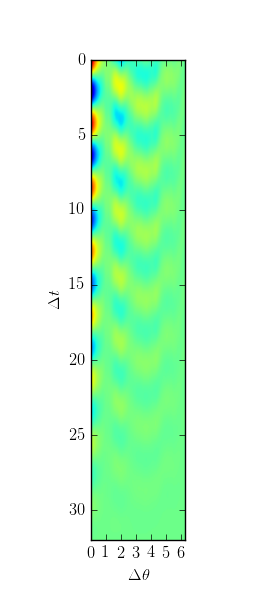
\includegraphics[width=0.3\textwidth]{circ-0p1-10-4}
}
\subfloat[][]{
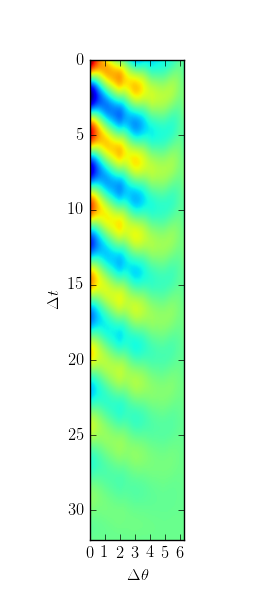
\includegraphics[width=0.3\textwidth]{circ-0p2-10-4}
}
\subfloat[][]{
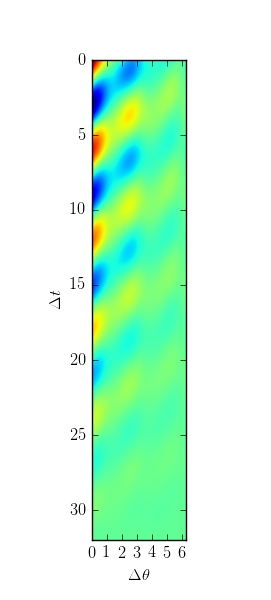
\includegraphics[width=0.3\textwidth]{circ-0p3-10-4}
}
\qquad
\subfloat[][]{
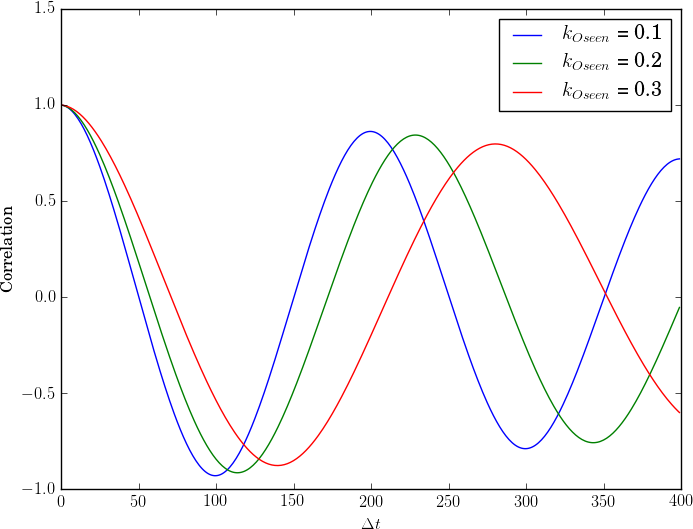
\includegraphics[width=0.5\textwidth]{circ_tcorrs_oseen_10-4}
}
\caption{Full correlation functions for circular geometry with $H=1$
and $k_{stiff}=10$, with $k_{Oseen}=$ 0.1, 0.2, and 0.3 (a-c,
respectively). The correlation function at $\Delta i = 0$ for all
of these values of $k_{Oseen}$ are shown in (d).  
\label{fig:oseenk}
}
\end{figure*}
The strength of the interaction tensor, $k_{Oseen}$, has a dramatic
effect on the type of wave behavior seen, or whether it is observed
at all. This strength is a function of the hydrodynamic effects of
kinesin walking along microtubules, and will depend on their density
and speed, as explained in detail in Ref. \cite{Monteith2016}. 
Figure \ref{fig:oseenk} shows the correlation results of
three 128-polymer simulations in the same circular geometry shown
in Figure \ref{fig:anims}(a) for three different values of $k_{Oseen}$.
There is an overall strengthening of the metachronal
behavior as $k_{Oseen}$ is increased from  $0.1$ to $0.2$. 
The sign of the slope reflects the initial conditions of the system.
Long lived waves travel predominantly in a single direction over
long times scales resulting in a 
slope of the crests of the correlation function that can
either be positive or negative. Similar crests are
seen in the analysis of the real experimental data~\cite{Sanchez2011}.
With this circular geometry, the correlation function must be periodic,
which is why it rises again when $i$ becomes large.
%Figs. \ref{fig:oseenk}(a-b) are more reminiscent of standard wavelike behavior.

\begin{figure*}
\centering
\subfloat[][]{
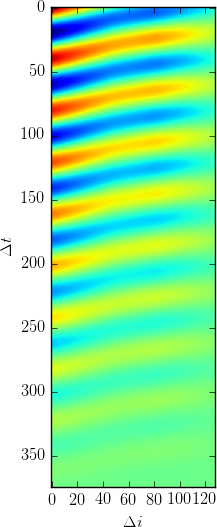
\includegraphics[width=0.3\textwidth]{plane-0p1-5-4}
}
\subfloat[][]{
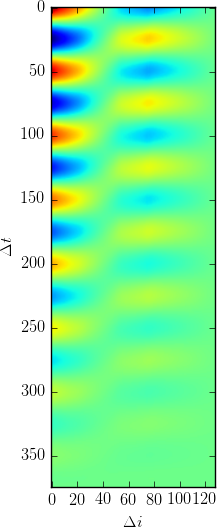
\includegraphics[width=0.3\textwidth]{plane-0p1-10-4}
}
\subfloat[][]{
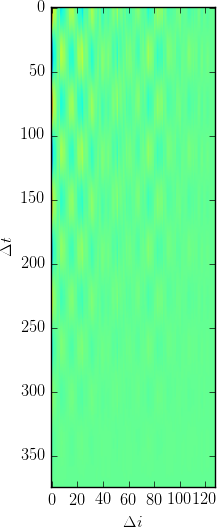
\includegraphics[width=0.3\textwidth]{plane-0p1-20-4}
}
\qquad
\subfloat[][]{
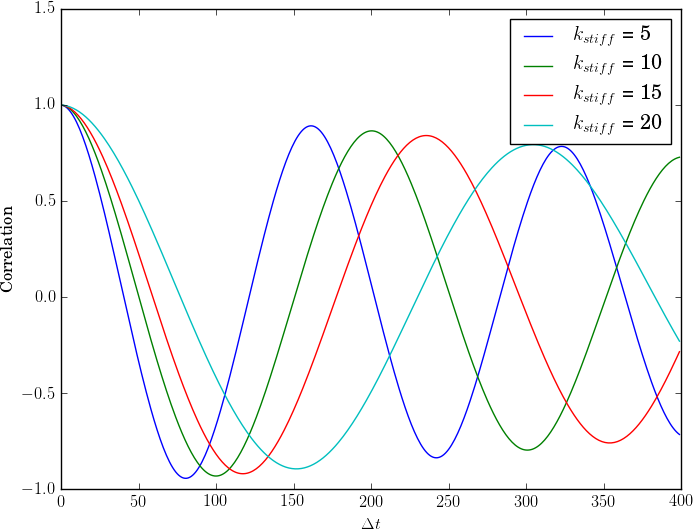
\includegraphics[width=0.5\textwidth]{plane_tcorr_stiff-0p1-4}
}
\caption{Full correlation functions for planar geometry with $H=1$
and $k_{Oseen}=0.1$, with $k_{stiff}=$ 5.0, 10.0, and 20.0 (a-c,
respectively). The correlation function at $\Delta i = 0$ for all
of these values of $k_{stiff}$ are shown in (d).  
\label{fig:stiffk}
}
\end{figure*}

The polymer stiffness $k_{stiff}$ also has an interesting effect
on metachronal wave formation. Figure \ref{fig:stiffk} shows the
correlation functions for $k_{stiff}=$ 5.0, 10.0, and 20.0 in a
planar geometry. While Figs. \ref{fig:stiffk}(a-b) are qualitatively
similar, we do see an apparent decrease in the metachronal wavelength.
Figs. \ref{fig:stiffk}(c-d) show that if the polymer is made too
stiff, no metachronal behavior is observed at all.
In general, planar geometry appears to cause more coherence in the motion of the different
bundles, and the correlation function is dominated by motion at
the longest lengths and time scales. 

\begin{figure*}
\centering
\subfloat[][]{
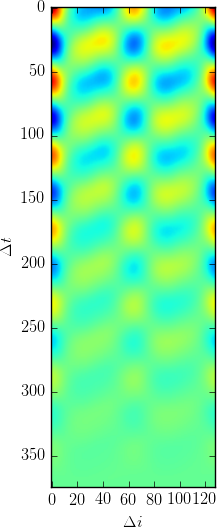
\includegraphics[width=0.3\textwidth]{circ-1H-0p2-10-4}
}
\subfloat[][]{
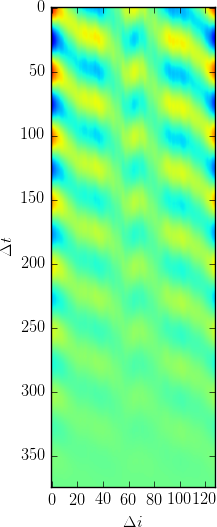
\includegraphics[width=0.3\textwidth]{circ-p5H-0p2-10-4}
}
\subfloat[][]{
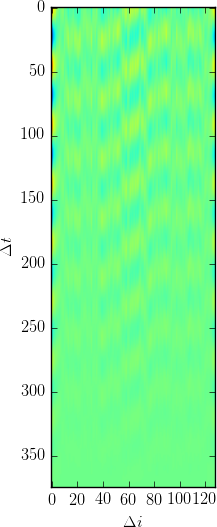
\includegraphics[width=0.3\textwidth]{circ-p1H-0p2-10-4}
}
\qquad
\subfloat[][]{
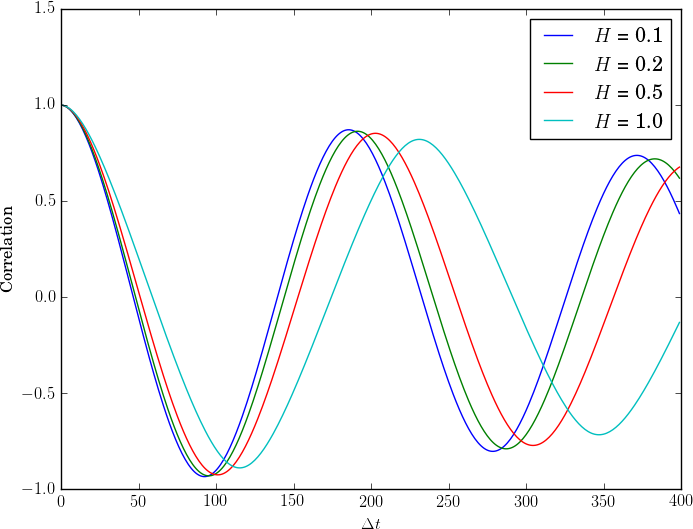
\includegraphics[width=0.5\textwidth]{circ_tcorr_H-0p2-10-4}
}
\caption{Full correlation functions for circular geometry with
$k_{stiff}=10$, $k_{Oseen}=0.2$, and $H$ = 1.0, 0.5, and 0.1 (a-c,
respectively). The correlation function at $\Delta i = 0$ for all
of these values of $H$ are shown in (d).  
\label{fig:H}} 
\end{figure*}


The distance between plates, $H$, has a considerable effect on the dynamics
as well. Longer range, more coherent motion is observed when $H$ is larger, and
short range, less coherent motion when $H$ is small. See Figure \ref{fig:H}. This
is to be expected due to the strong screening effect that these boundary conditions
impose. Smaller $H$ reduces the hydrodynamic coupling, causing a decrease in coherence.

%------------------------------------------------

\section{Discussion}
\label{sec:disc}
When comparing these results to those of
Sanchez et al., we find that the basic features agree. The videos
included in the supplemental materials qualitatively mimic the
experimental videos, and the experimental correlation analysis
agrees quite well with the simulations. More importantly, this agreement between
theory and experiment was reached from first principles. We only
use a handful of forces in our simulations, and each force has a
physical justification for being used.

There are potential shortcomings of this model that may result in
some differences between experiment and theory. 
The first is that the experiments observe bundles of microtubules
that taper away from their base. The hydrodynamics are not
expected to be uniform along the length of a chain. In addition
these bundles will, for short enough times, behave like rigid
material, but for longer times, because they are connected through
walking kinesin molecules, will behave more as individual mictrotubules
with a greatly reduced elastic constant. On the time scales of the motion,
we expect to be in the latter regime. However the details of the
hydrodynamics and elasticity in these bundles is still not understood
experimentally. In fact, as we mentioned earlier, the polarity of
individual MT's is not known experimentally, and arguments for their
unipolarity are given in \ref{app:unipolar}.
But still, the basic mechanism of dynamic buckling due to kinesin drag, 
and metachronal waves being generated by hydrodynamic coupling is
robust over a wide parameter range, so we believe that these
complications, aside from unipolarity, will not alter the basics of our explanation.

At a more technical level, there are other things that may
make a slight difference to the results here.
The bundles are constrained to move only in the $xy$-plane, and
while it is true that MT motion is nearly 2-dimensional, there is
some room in the $z-$direction that MT bundles can occupy. Additionally,
this model does not account for the fluid boundary condition at the
anchoring surface. This may introduce some errors if a monomer
becomes close ($\sim H$) to the anchoring plane. However, because
of the screening effects of the plates, this should not alter the behavior
at distances large compared to the plate separation. We have tested
for this by adding image charges to the planar case, 
and found that their effects on correlations are small, as expected.

\section{Conclusions}
In conclusion,
we have developed a model for the spontaneous formation of wavelike
behavior in active polymer arrays that only requires two ingredients:
semi-flexible chains tethered to a surface, and motors walking from
their bases to their tips. The hydrodynamics in their confined
geometry gives rise to metachronal waves that appear remarkably
similar to what is observed experimentally~\cite{Sanchez2011,sanchez2013engineering}.
There is no need to posit additional mechanisms that force
individual bundles to oscillate. This all happens as a consequence of Newton's
laws and fluid mechanics, allowing us to
gain a better understanding of how metachronal waves form with
considerable predictive power. As such, we have examined new parameter spaces and have
demonstrated boundaries between different types of metachronal
behavior and regimes in which no metachronal behavior exists.
It would be of great interest to test these predictions
experimentally.
Given the simplicity and robust nature of this mechanism, 
and the ubiquity of microtubules and kinesin in cells, it
gives one further impetus to look for other places in biology
where this kind of behavior can be found.


\chapter{Spontaneous Circulation of Active Microtubules Confined by Optical Traps}

\chapter{Conclusion}

\nocite{*}
\bibliographystyle{unsrt}
\bibliography{Thesis}

\appendix
\chapter{Supplementary Videos}
\noindent
Supplementary videos for the material in Chapter 3 can be found here:\\
\url{https://sites.google.com/ucsc.edu/joshdeutsch/metachronal-videos?authuser=0}\\ \\
Supplementary videos for the material in Chapter 4 can be found here:



\end{document}
